\documentclass[10pt]{beamer}

\usetheme[]{JuanLesPins}
\setbeamercolor{structure}{fg=brown}
\setbeamertemplate{navigation symbols}{}
\setbeamertemplate{footline}[frame number]
%-------------------------------------------------------
% INCLUDE PACKAGES
%-------------------------------------------------------

\usepackage[utf8]{inputenc}
\usepackage[francais]{babel}
\usepackage[T1]{fontenc}
\usepackage{helvet}
\usepackage{graphicx}
\usepackage{amsmath,amsfonts,amssymb}
\usepackage{enumitem}
\usepackage{float}
\usepackage{hyperref}
\usepackage{cases}
\usepackage[justification=centering]{caption}
%\usepackage{media9}
%\usepackage{movie15}
\usepackage{multimedia}
\usepackage{url}
\AtBeginSection[]{
  \begin{frame}
  \vfill
  \centering
  \begin{beamercolorbox}[sep=8pt,center,shadow=true,rounded=true]{title}
    \usebeamerfont{title}\insertsectionhead\par%
  \end{beamercolorbox}
  \vfill
  \end{frame}
}

\AtBeginSection[]
{
	\begin{frame}{Plan}
		\tableofcontents[currentsection]
	\end{frame}
}


%-------------------------------------------------------
% INFORMATION IN THE TITLE PAGE
%-------------------------------------------------------

\title[Population Néanderthal]{\textbf{Evolution de la population \\ d'\textit{Homo Néanderthalensis}}}
\author[Y. Adimy, M. Simon, H. Vassal]{Y. Adimy M. Simon H. Vassal}
\institute[]{INSA Lyon - Bioinformatique et Modélisation}
\date{13 Juin 2016}
\titlegraphic{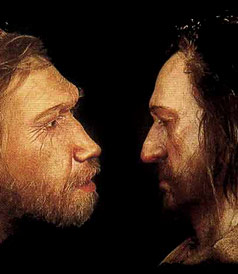
\includegraphics[width=3cm]{neanderthal-sapiens.jpg}}
\logo{
\includegraphics[scale=0.1]{logo_insa.png}}

%-------------------------------------------------------
% THE BODY OF THE PRESENTATION
%-------------------------------------------------------

\begin{document}

%-------------------------------------------------------
% THE TITLEPAGE
%-------------------------------------------------------

\begin{frame}[plain,noframenumbering] 
   \titlepage
   \insertlogo
\end{frame}

%\frame[plain,noframenumbering]{\tableofcontents}





\section{Introduction}
\subsection{La disparition mystérieuse de Néandertal}
\begin{frame}{La disparition mystérieuse de Néandertal}
	\begin{columns}
		\begin{column}{6cm}
			\begin{figure}[L]
				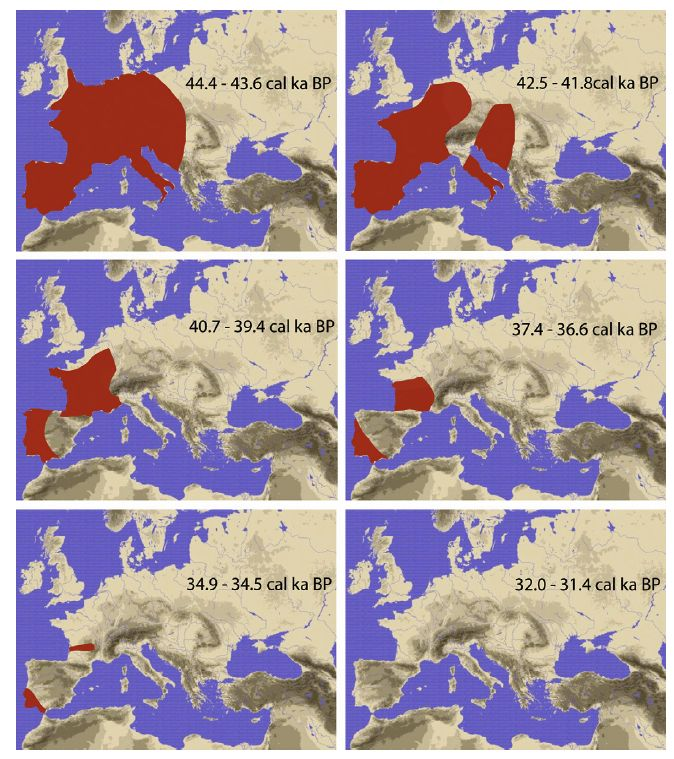
\includegraphics[width=0.8\linewidth]{Carte}\vfill
				\caption{Régions occupées par Néandertal à différentes époques en Europe}
			\end{figure}
		\end{column}
		\begin{column}{6cm}
			\begin{figure}[R]
				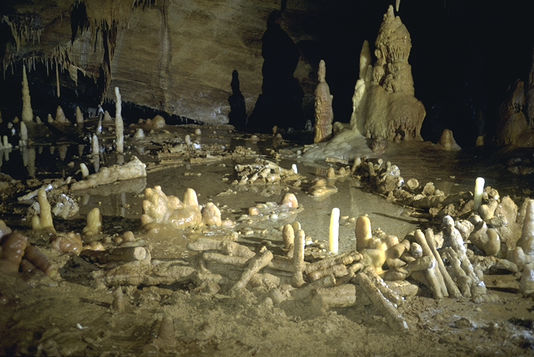
\includegraphics[width=0.8\linewidth]{GrotteBrunel} \vfill 
				\caption{La grotte de Bruniquel, plus ancienne construction humaine }
			\end{figure}
		\end{column}
	\end{columns}
\end{frame}	




\subsection{Cadre général}

\begin{frame}{Cadre général}{}
\begin{block}{Modèle général}
	\begin{equation}
		\frac{\partial u(t,x)}{\partial t}=f(u(t,x))+d\Delta u(t,x),
	\end{equation}
	\vspace{0.1cm}
	$$	\quad t \in \mathbb{R}, \quad x \in \mathbb{R}^n, \quad n=1 \text{ ou } n=2,$$

	
\end{block}
\begin{itemize}
	\item u(t,x) : Densité de population à la position x et au temps t. 
    \item $d$ : Constante de diffusion. 
    \item $f$ : Terme de réaction.
\end{itemize}
\end{frame}

\section{Croissance logistique}
\subsection{Présentation du modèle}
\begin{frame}{Présentation du modèle}{}
\begin{block}{Croissance Logistique}
	$$\frac{\partial u(t,x)}{\partial t}=\alpha  u(t,x) \left( 1 - \dfrac{u(t,x)}{K}\right) +d\Delta u(t,x),$$
\end{block}
\begin{itemize}
    \item $K$ : Capacité du milieu liée à des facteurs locaux environnementaux ($K> 0$).
    \item $\alpha$ : Taux de croissance intrinsèque de la population ($\alpha >0$).
\end{itemize}
\end{frame}

\subsection{Analyse mathématique}
\begin{frame}{Analyse mathématique}
	\begin{block}{Analyse de la partie réaction}
	 0 équilibre instable et K équilibre stable
		
	\end{block}
	
	\begin{block}{Analyse de l'équation de réaction-diffusion}
	 L'équation de réaction diffusion est de type \textbf{KPP monostable}.
		\begin{itemize}
		
			\item[$\bullet$] Pour tout $c> 2 \sqrt{\alpha}$ il existe un unique front d'onde U(z) monotone se propageant à la vitesse c tel que $lim_{z \to + \infty}U(z) =0$ et  $lim_{z \to - \infty} U(z)=K$.

			
			\item[$\bullet$] Effet \textit{"hair trigger"}: Si on prend une condition initiale positive sur un intervalle borné et nul en dehors de l'intervalle, alors la solution converge vers K à la vitesse $2\sqrt{\alpha}$.
			
		\end{itemize}
	\end{block}	
	
	

\end{frame}


\subsection{Simulations numériques}

\begin{frame}{Propagation d'un front d'onde en 1D}{}
	\begin{figure}[H]
		\centering
		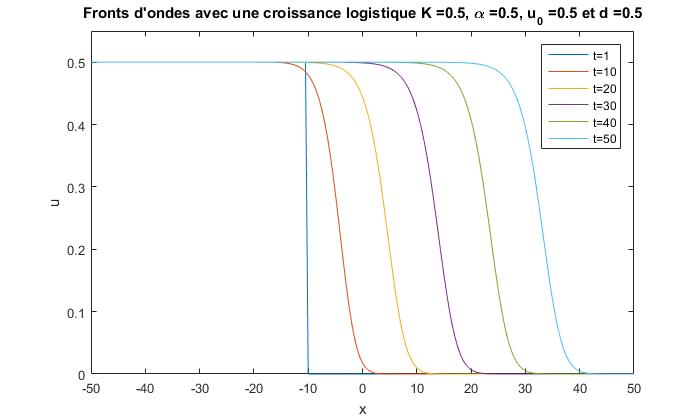
\includegraphics[width=0.55\linewidth]{SimulationKPP/figures1/FrontOnde2}\hfill
		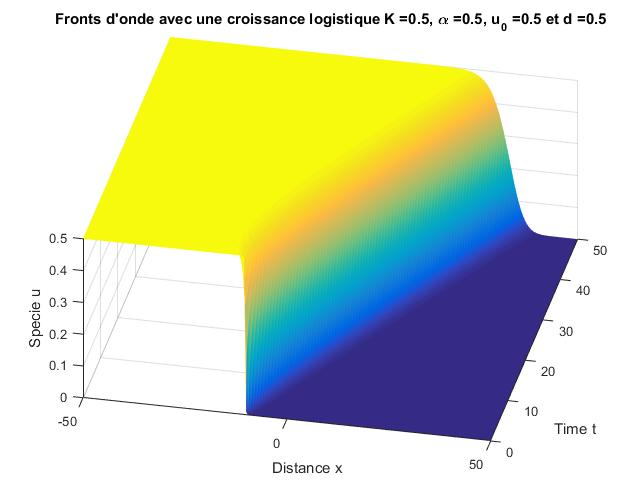
\includegraphics[width=0.40\linewidth]{SimulationKPP/figures1/FrontOnde1}\hfill
		\caption{Propagation du front d'onde en 1D ( \url{KPP1D.avi})}
	\end{figure}
\end{frame}



\begin{frame}{Effet "hair trigger"}{}
\begin{figure}[H]
	\centering
	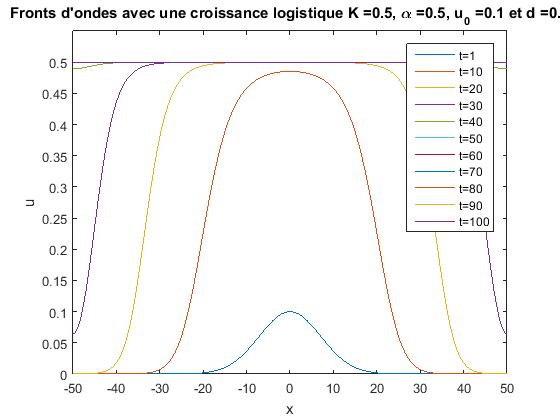
\includegraphics[width=0.45\linewidth]{SimulationKPP/TrigerEffect/fronts}\hfill
	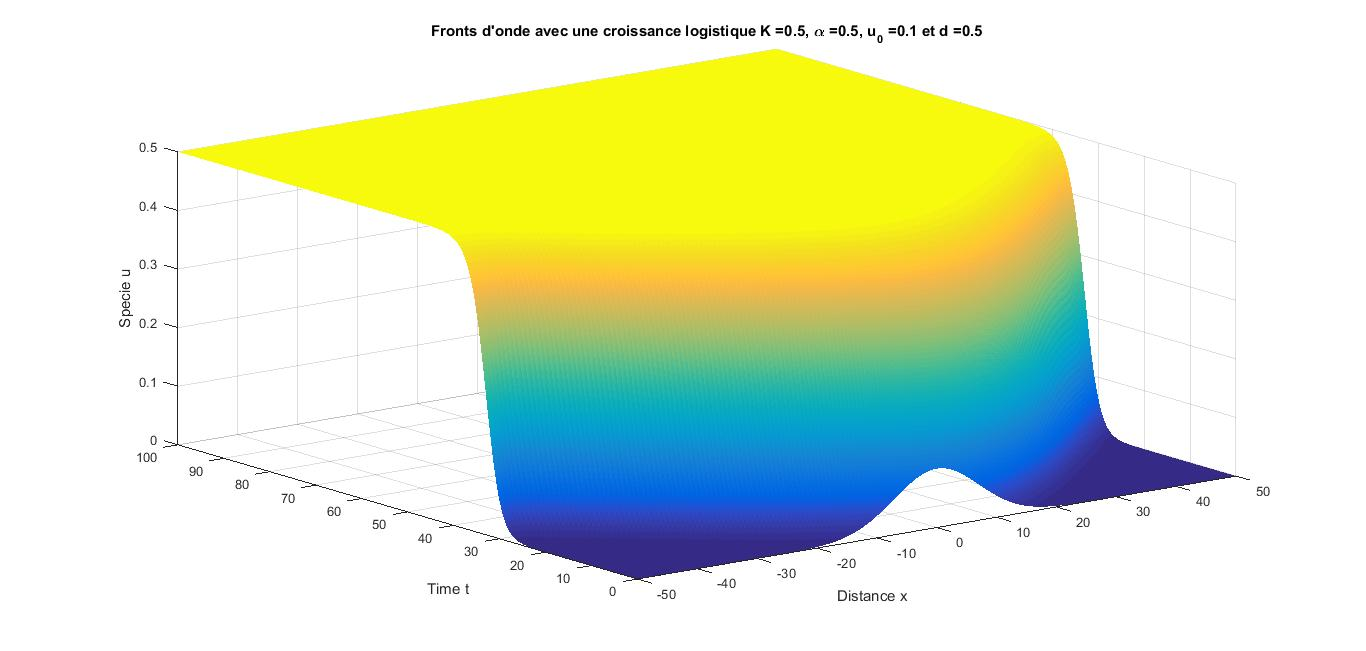
\includegraphics[width=0.55\linewidth]{SimulationKPP/TrigerEffect/Surf}\hfill
	\caption{Propagation du front d'onde en 1D avec une petite perturbation initiale à support compact.}
\end{figure}
\end{frame}

\begin{frame}{Effet d'une barrière géographique franchissable}{}
\begin{figure}[H]
	\centering
	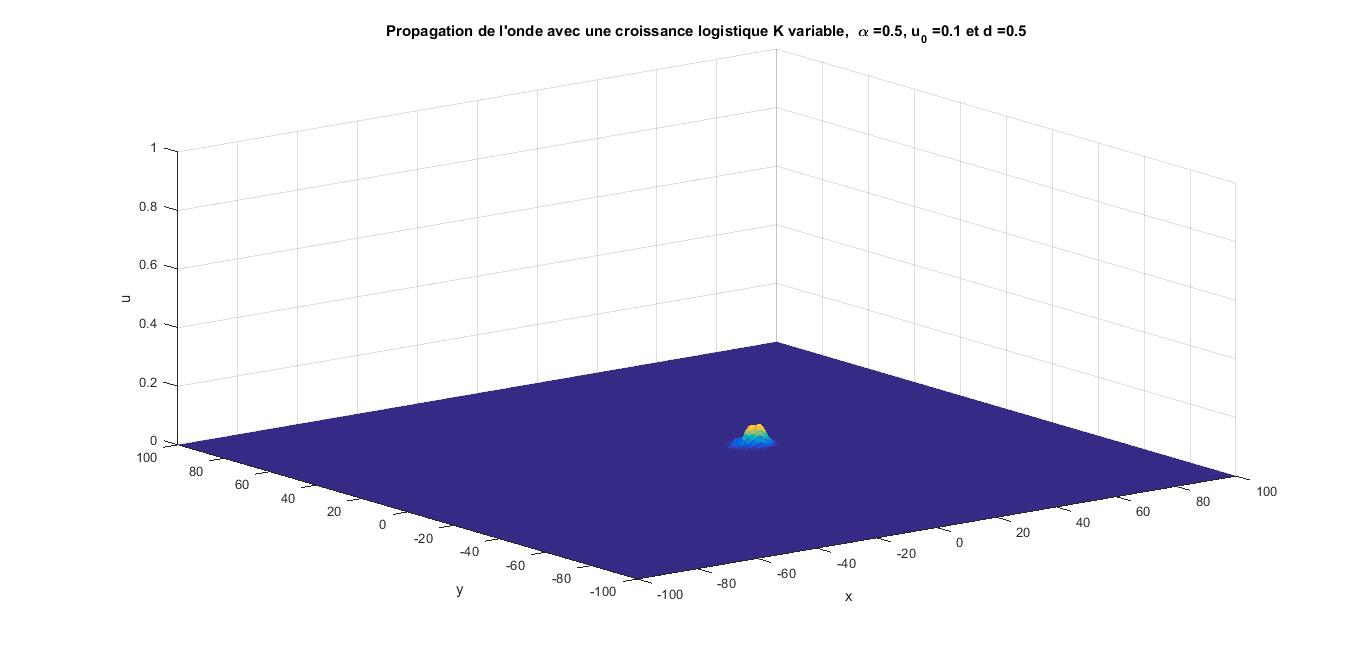
\includegraphics[width=0.5\linewidth]{SimulationKPP/Enviro/montagne1}\hfill
	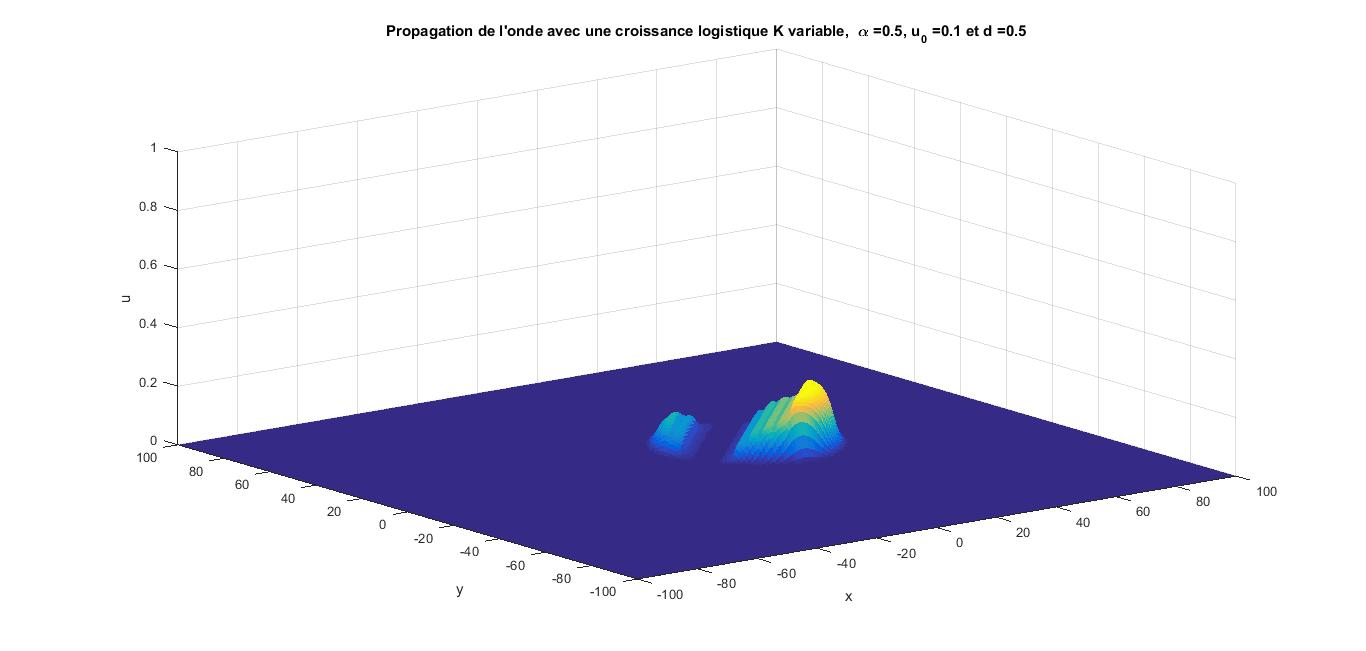
\includegraphics[width=0.5\linewidth]{SimulationKPP/Enviro/montagne3}\hfill
	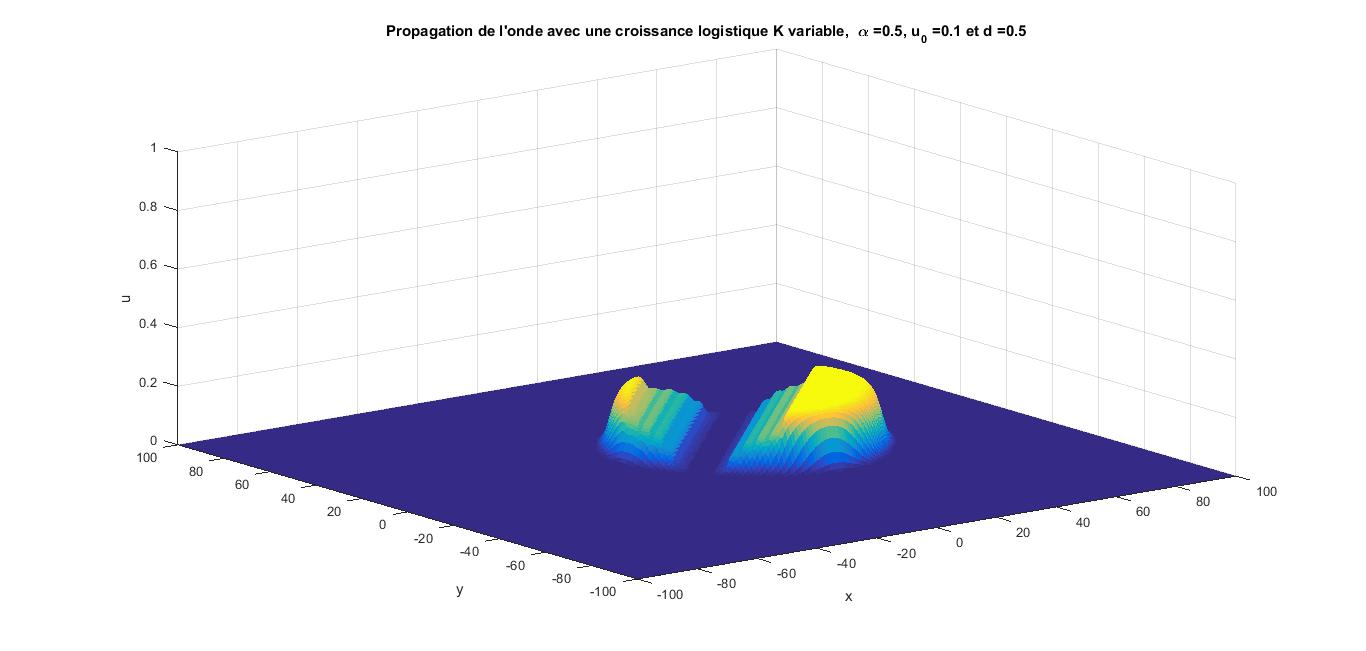
\includegraphics[width=0.5\linewidth]{SimulationKPP/Enviro/montagne5}\hfill
	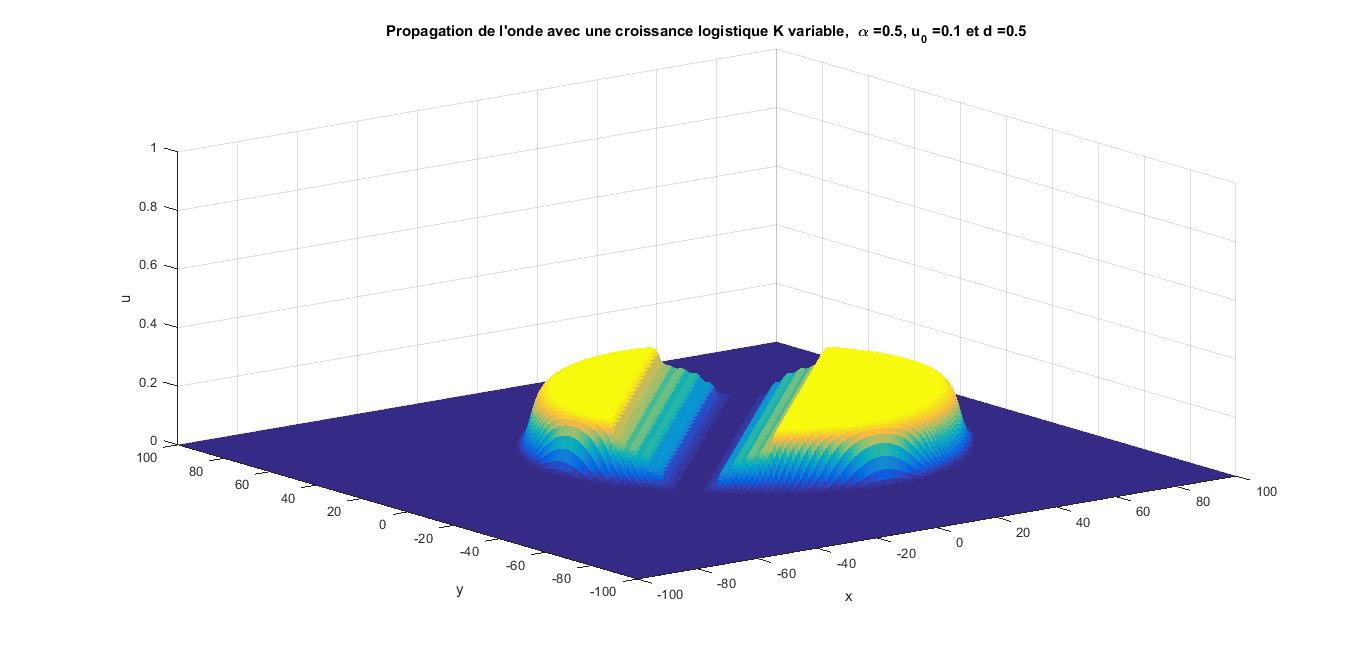
\includegraphics[width=0.5\linewidth]{SimulationKPP/Enviro/montagne8}
	\caption{Diffusion 2D de la population face à une barrière géographique franchissable : \url{KPPFranchissable.avi}}
\end{figure}
\end{frame}

\begin{frame}{Effet d'une barrière géographique infranchissable}{}
\begin{figure}[H]
	\centering
	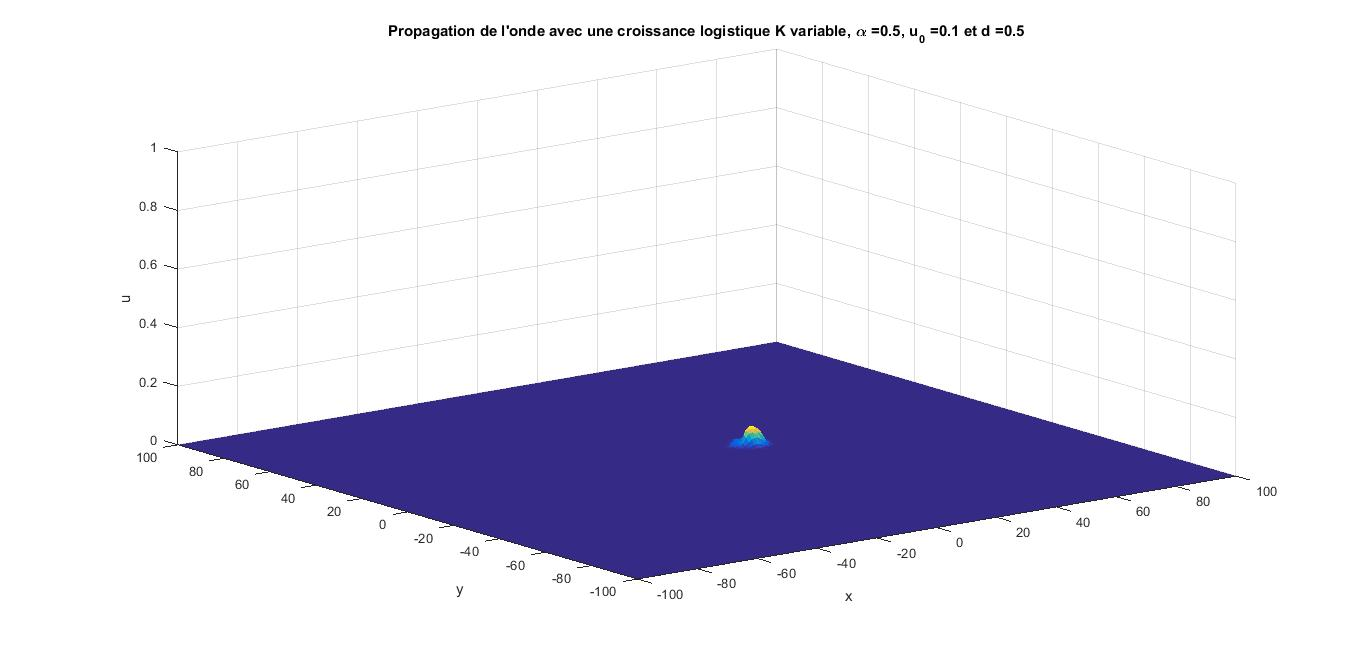
\includegraphics[width=0.5\linewidth]{SimulationKPP/Enviro/poleNord1}\hfill
	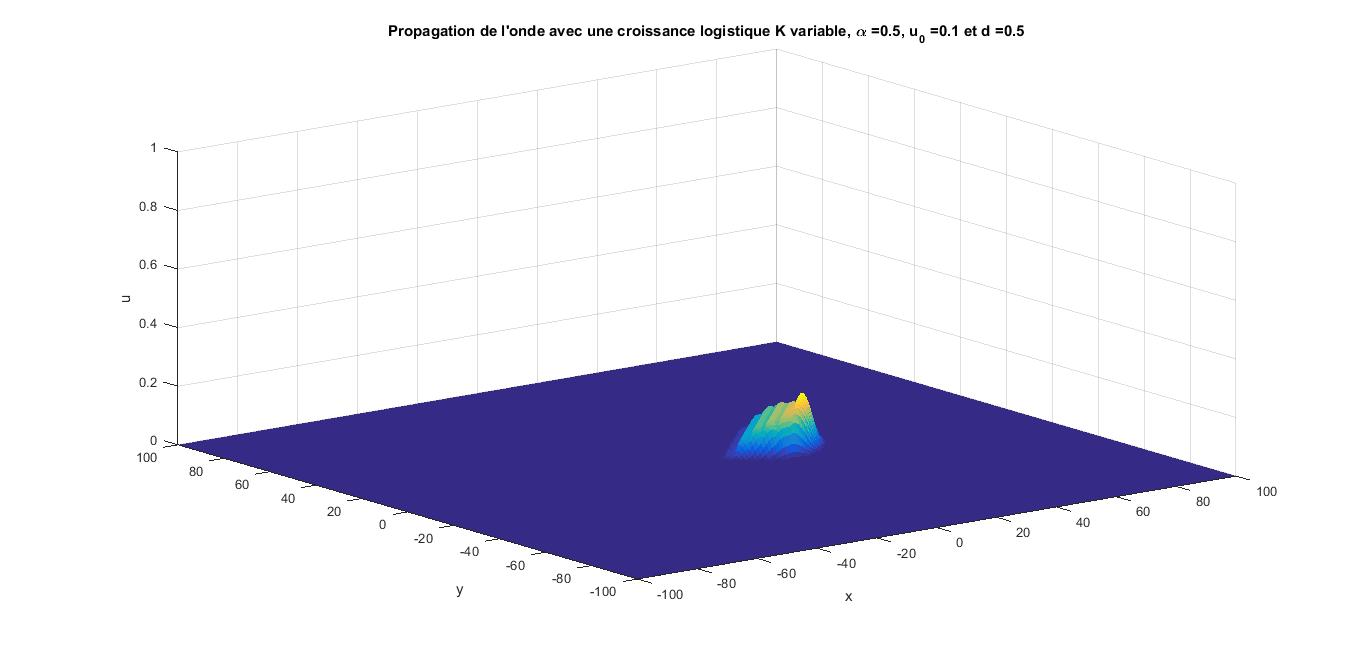
\includegraphics[width=0.5\linewidth]{SimulationKPP/Enviro/poleNord3}\hfill
	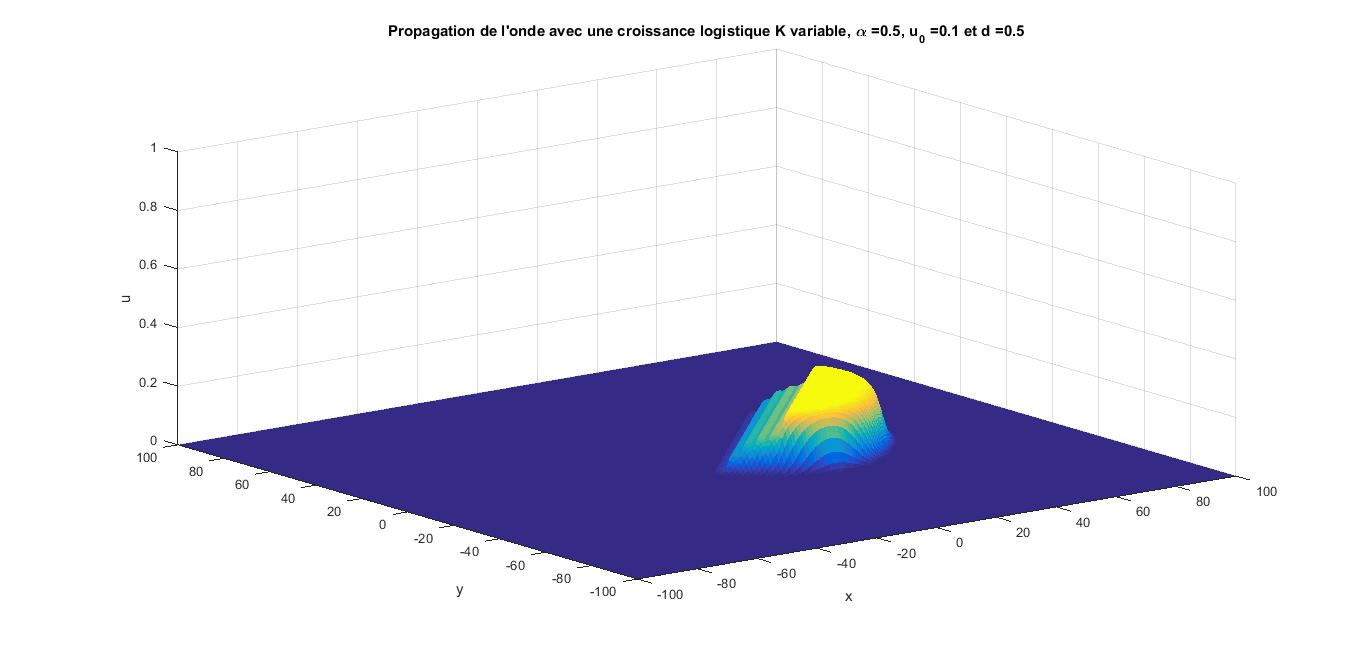
\includegraphics[width=0.5\linewidth]{SimulationKPP/Enviro/poleNord5}\hfill
	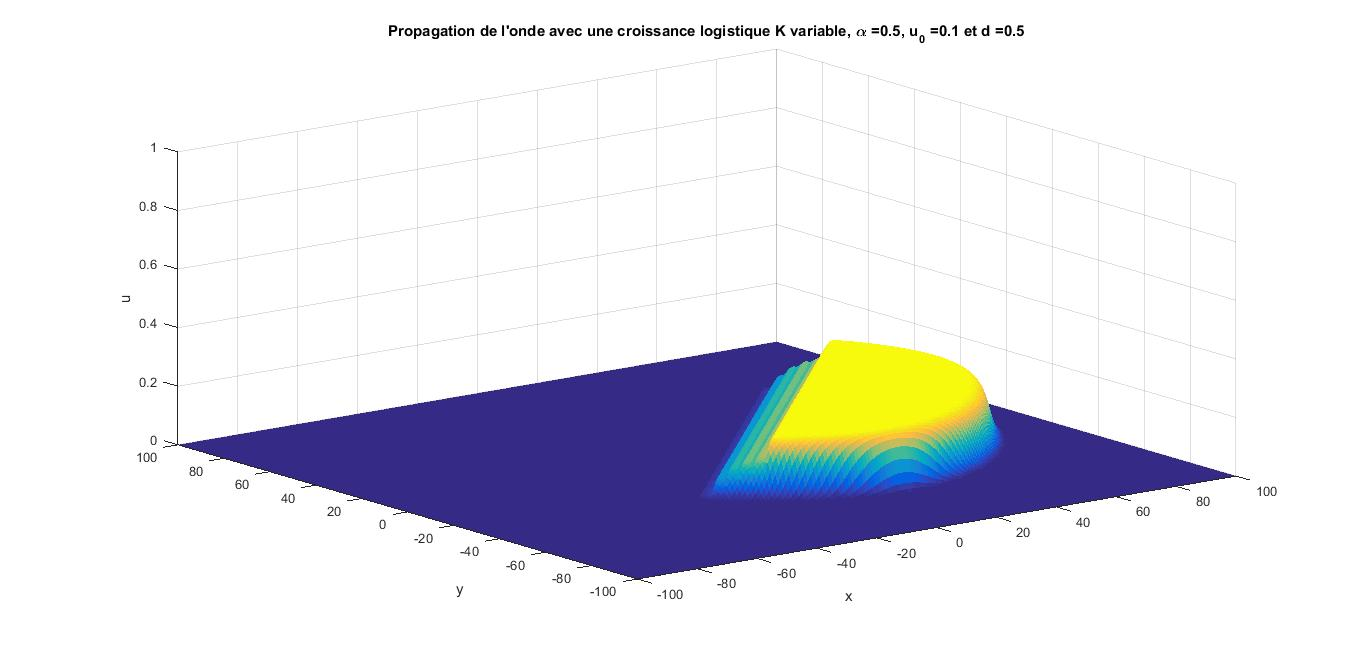
\includegraphics[width=0.5\linewidth]{SimulationKPP/Enviro/poleNord8}
	\caption{Diffusion 2D de la population face à une barrière géographique infranchissable : \url{KPPNonFranchissable.avi} }
	
\end{figure}

\end{frame}


\section{Effet Allee}
\subsection{Présentation du modèle}
\begin{frame}{Présentation du modèle}{}
\begin{block}{Modèle Allee}
	$$\frac{\partial u(t,x)}{\partial t}=f(u(t,x))+d\Delta u(t,x)$$
	$$f(u(t,x))=ku(1-u)(u-A)$$
\end{block}
\begin{itemize}
    \item $k$ : Taux de croissance normalisé constant 
    \item $A$ : Densité critique
\end{itemize}
$$k=\frac{4}{(1-A)^2}$$
\end{frame}

\subsection{Analyse mathématique}
\begin{frame}{Analyse mathématique}{}
\begin{itemize}
	\item[$\bullet$] Équilibres: $u=0, u=A \text{ et } u=1$
	\item[$\bullet$] BISTABLE
	\item[$\bullet$] 2 scénarios selon la valeur de A :
	\begin{itemize}
		\item[-] $A<0.5$ : $c>0$ $\rightarrow$ "1 envahit 0"
		\item[-] $A>0.5$ : $c<0$ $\rightarrow$ "0 envahit 1"
	\end{itemize}
\end{itemize}
\end{frame}

\subsection{Simulations numériques}
\begin{frame}{$\ d=0.5, A=0.25 (k=64), u_0=0.1$}{}
\begin{figure}[H]
	\centering
	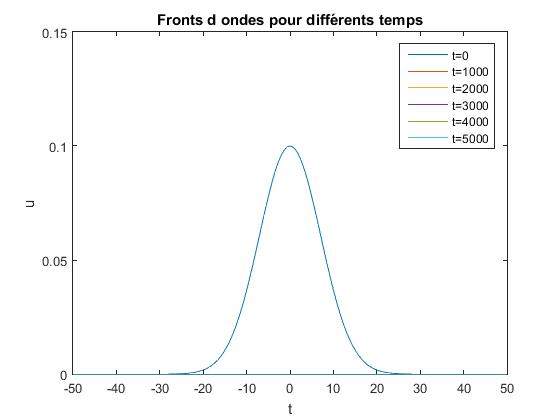
\includegraphics[width=0.40\linewidth, height=3cm]{Allee/F2311}\hfill
	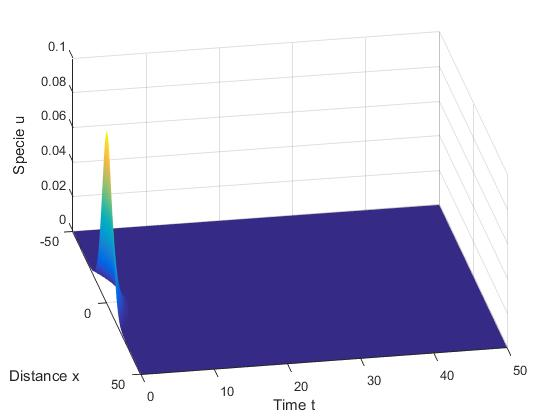
\includegraphics[width=0.55\linewidth, height=3cm]{Allee/F4311}
\end{figure}
\begin{figure}[H]
	\centering
	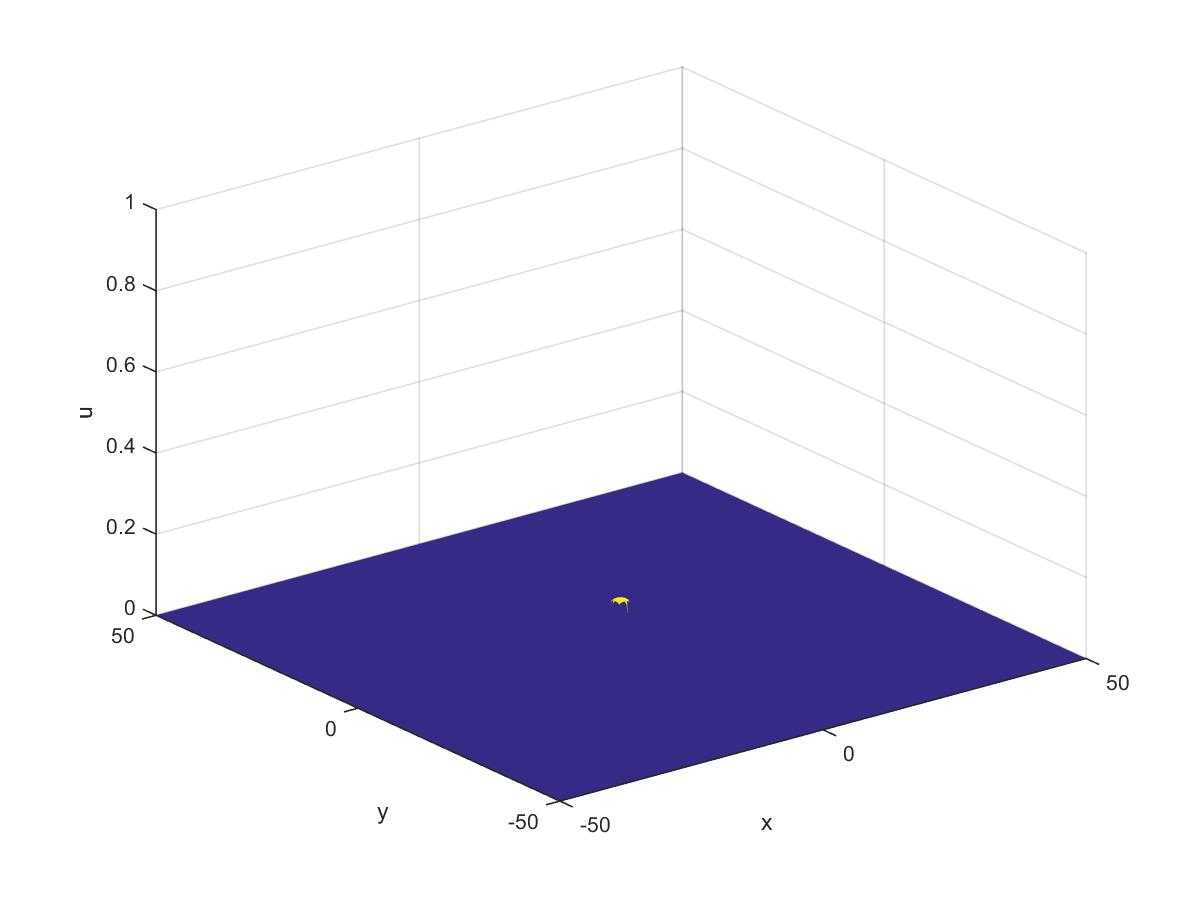
\includegraphics[width=0.3\linewidth]{Allee/311__1_}\hfill
    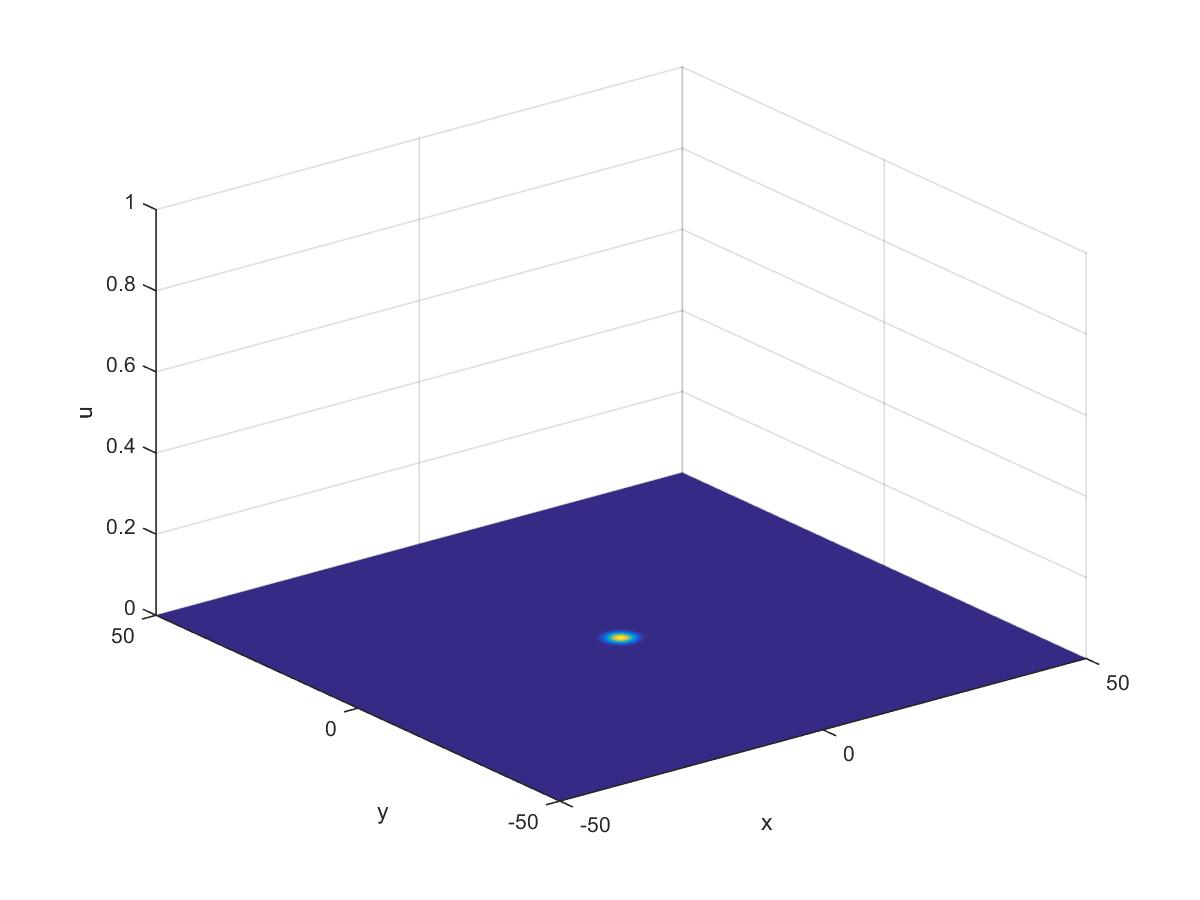
\includegraphics[width=0.3\linewidth]{Allee/311__2_}\hfill
	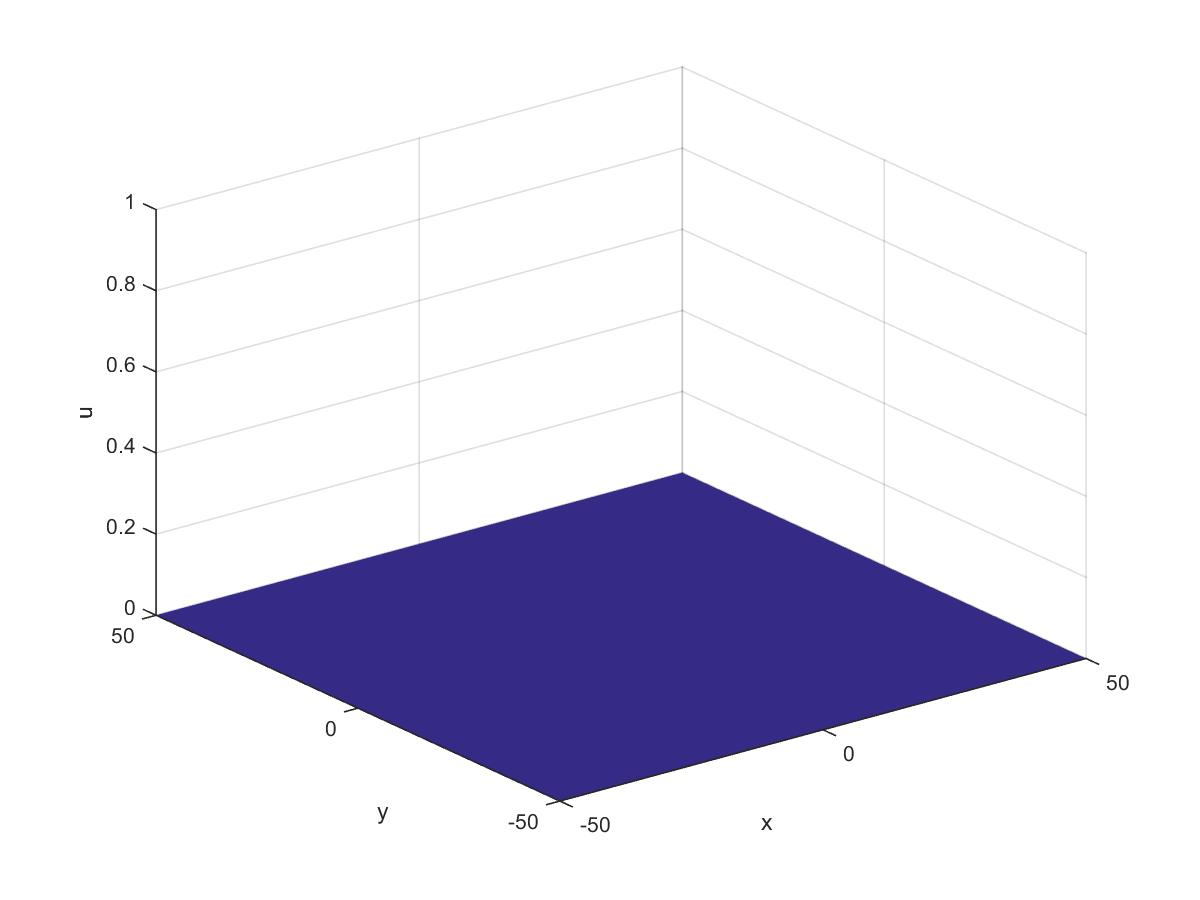
\includegraphics[width=0.3\linewidth]{Allee/311__3_}
\end{figure}
\end{frame}

\begin{frame}{$\ d=0.5, A=0.25 (k=64), u_0=0.5$}{}
\begin{figure}[H]
	\centering
	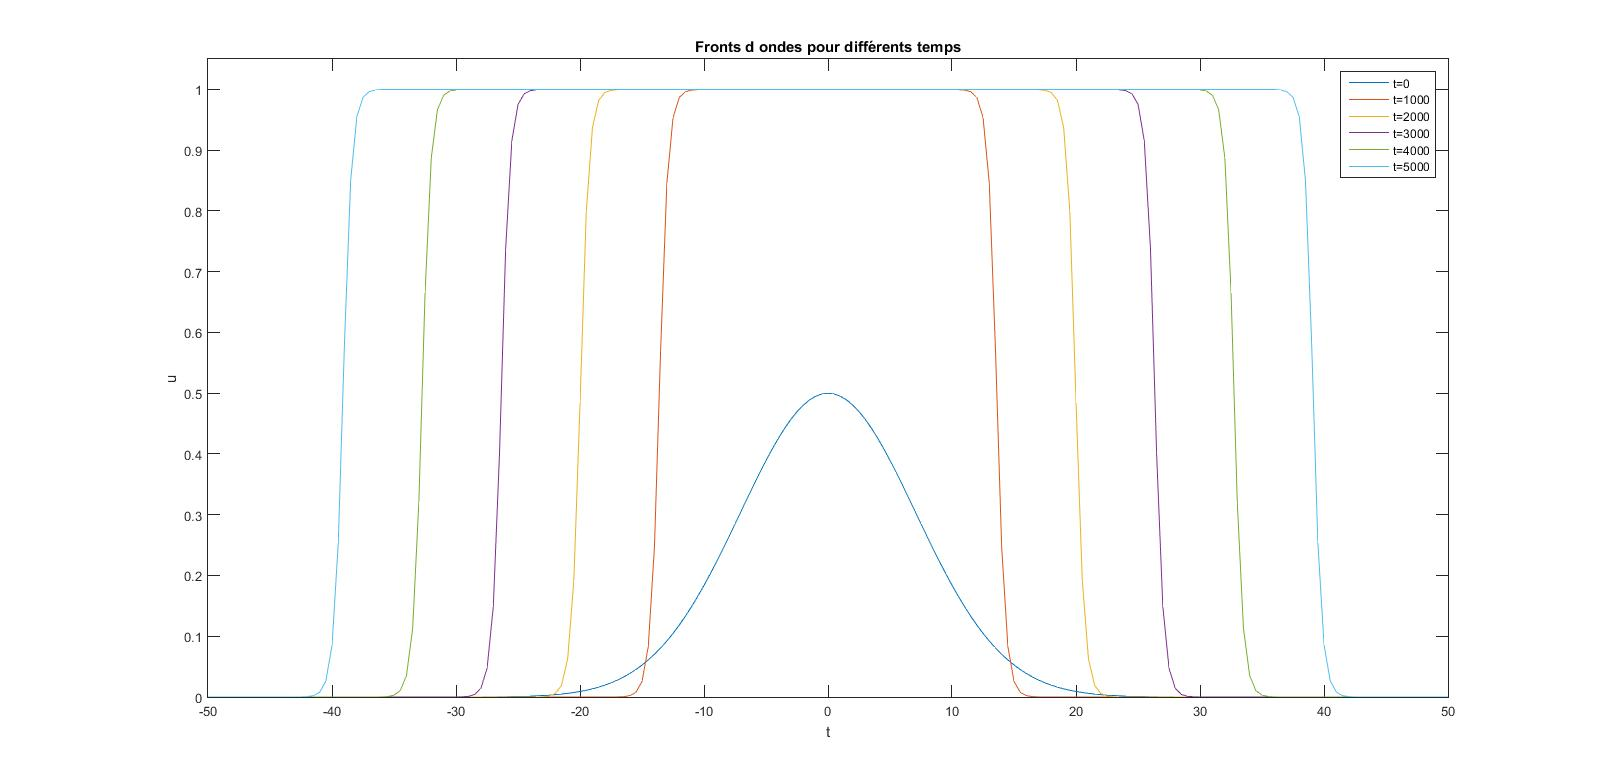
\includegraphics[width=0.40\linewidth, height=3cm]{Allee/F2312}\hfill
	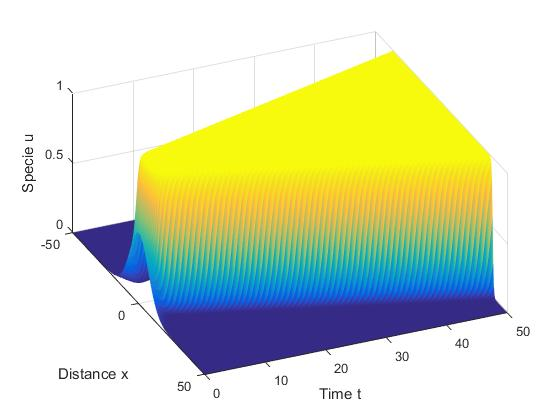
\includegraphics[width=0.55\linewidth, height=3cm]{Allee/F4312}
\end{figure}
\begin{figure}[H]
	\centering
	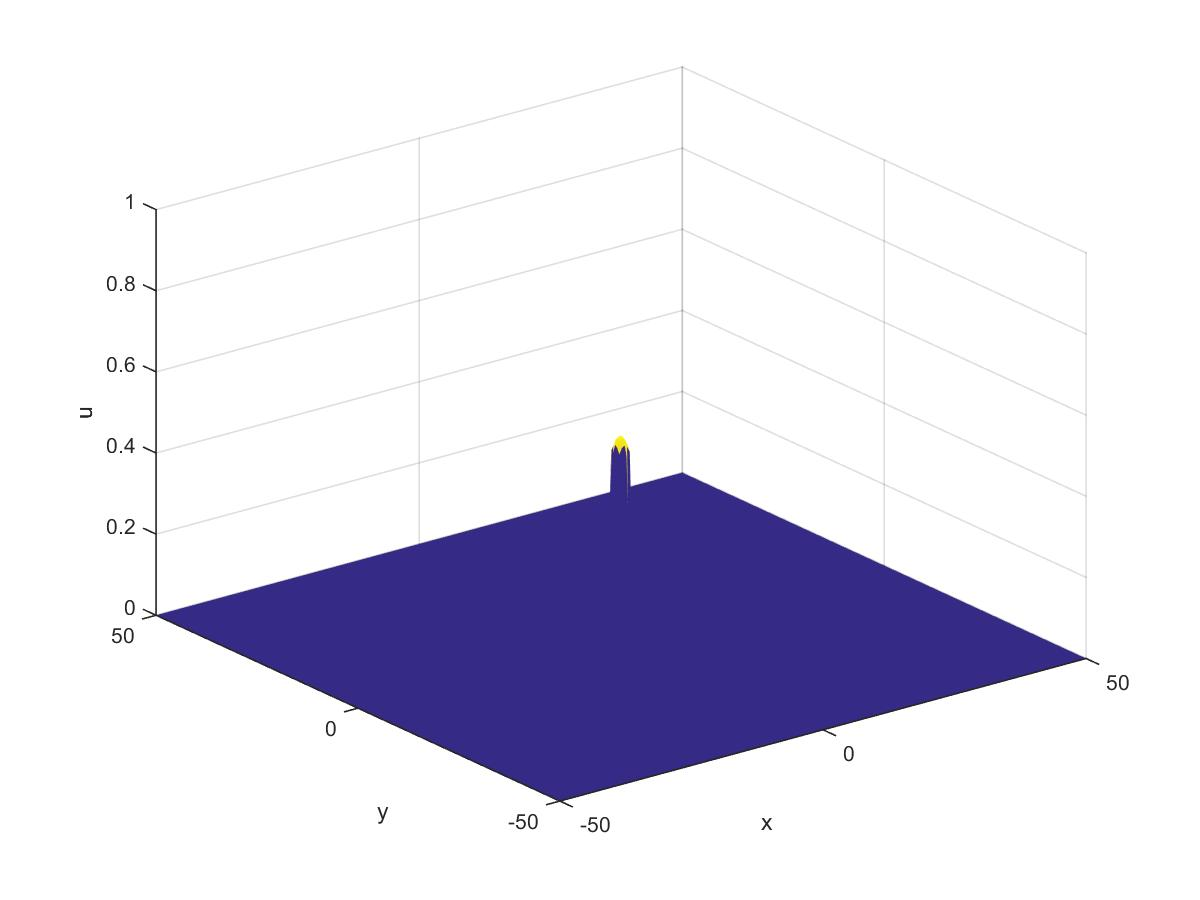
\includegraphics[width=0.3\linewidth]{Allee/312__1_}\hfill
    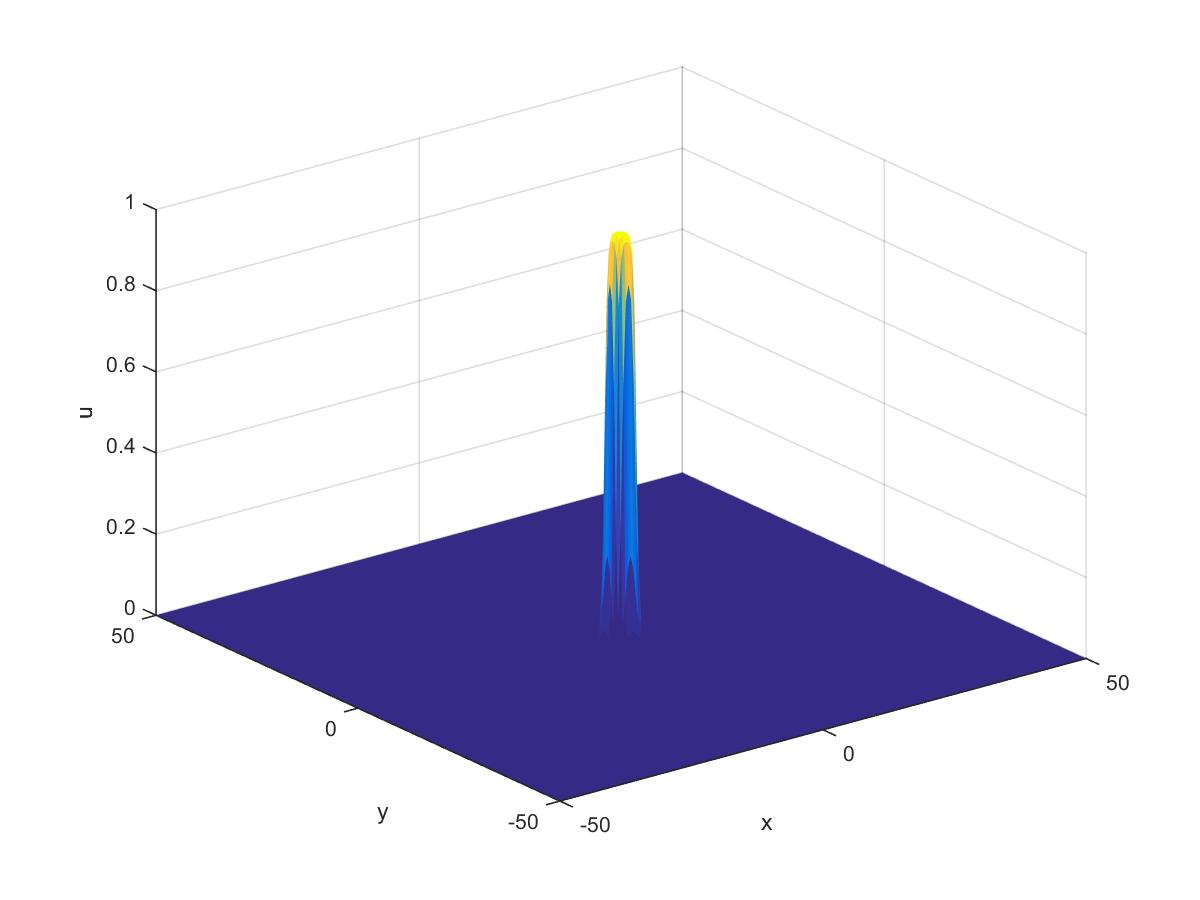
\includegraphics[width=0.3\linewidth]{Allee/312__2_}\hfill
	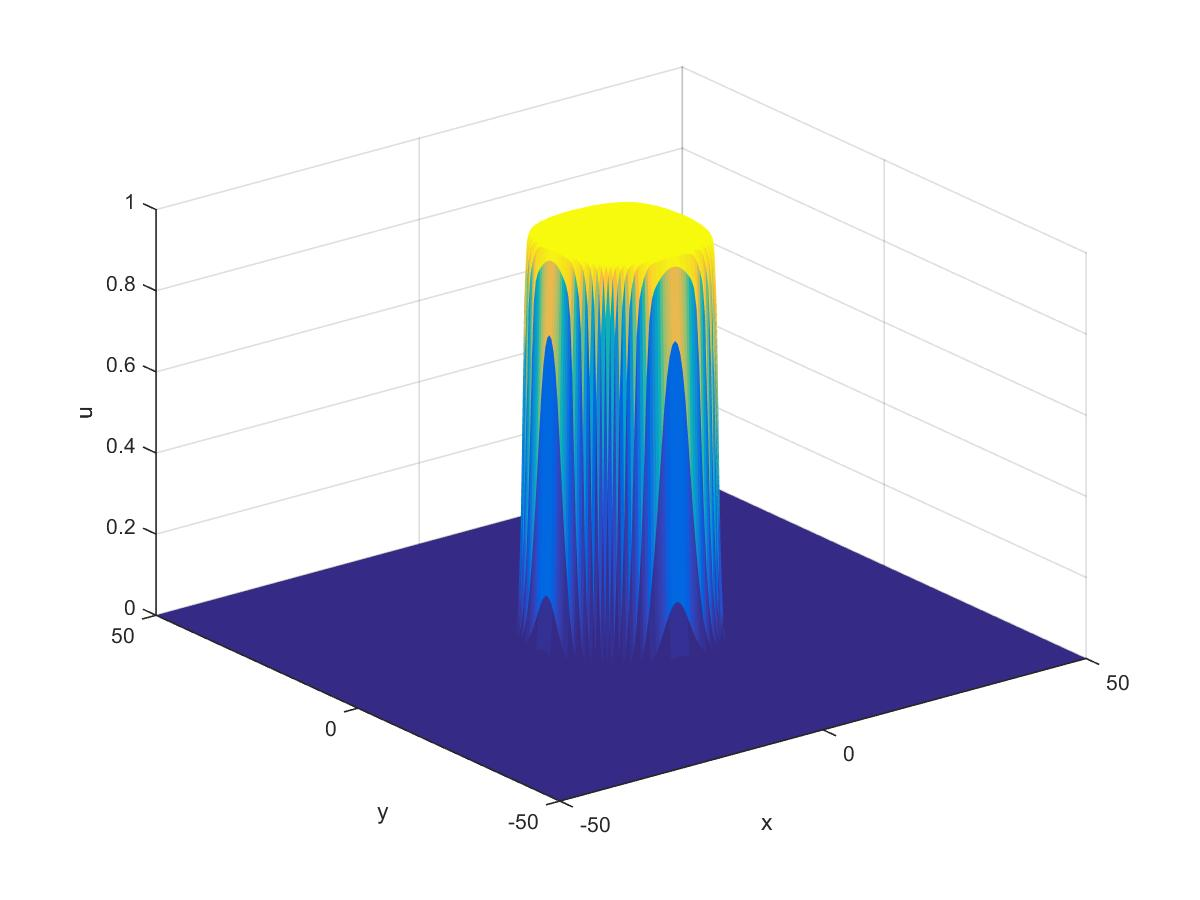
\includegraphics[width=0.3\linewidth]{Allee/312__3_}
\end{figure}
\end{frame}

\begin{frame}{$\ d=0.5, A=0.75 (k=7.1), u_0=0.5$}{}
\begin{figure}[H]
	\centering
	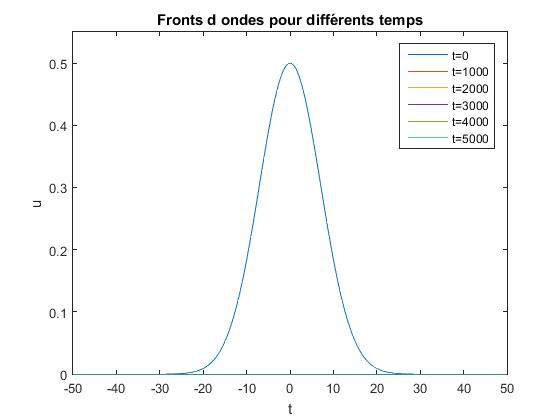
\includegraphics[width=0.40\linewidth, height=3cm]{Allee/F2322}\hfill
	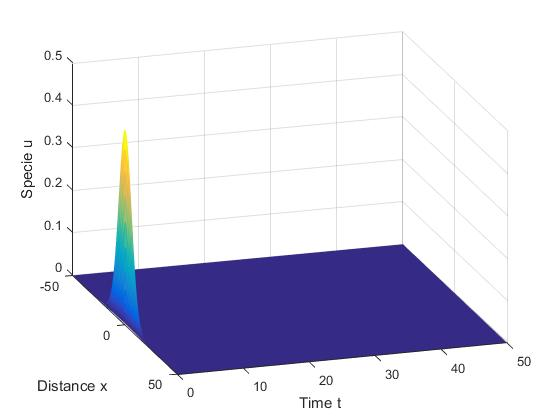
\includegraphics[width=0.55\linewidth, height=3cm]{Allee/F4322}
\end{figure}
\begin{figure}[H]
	\centering
	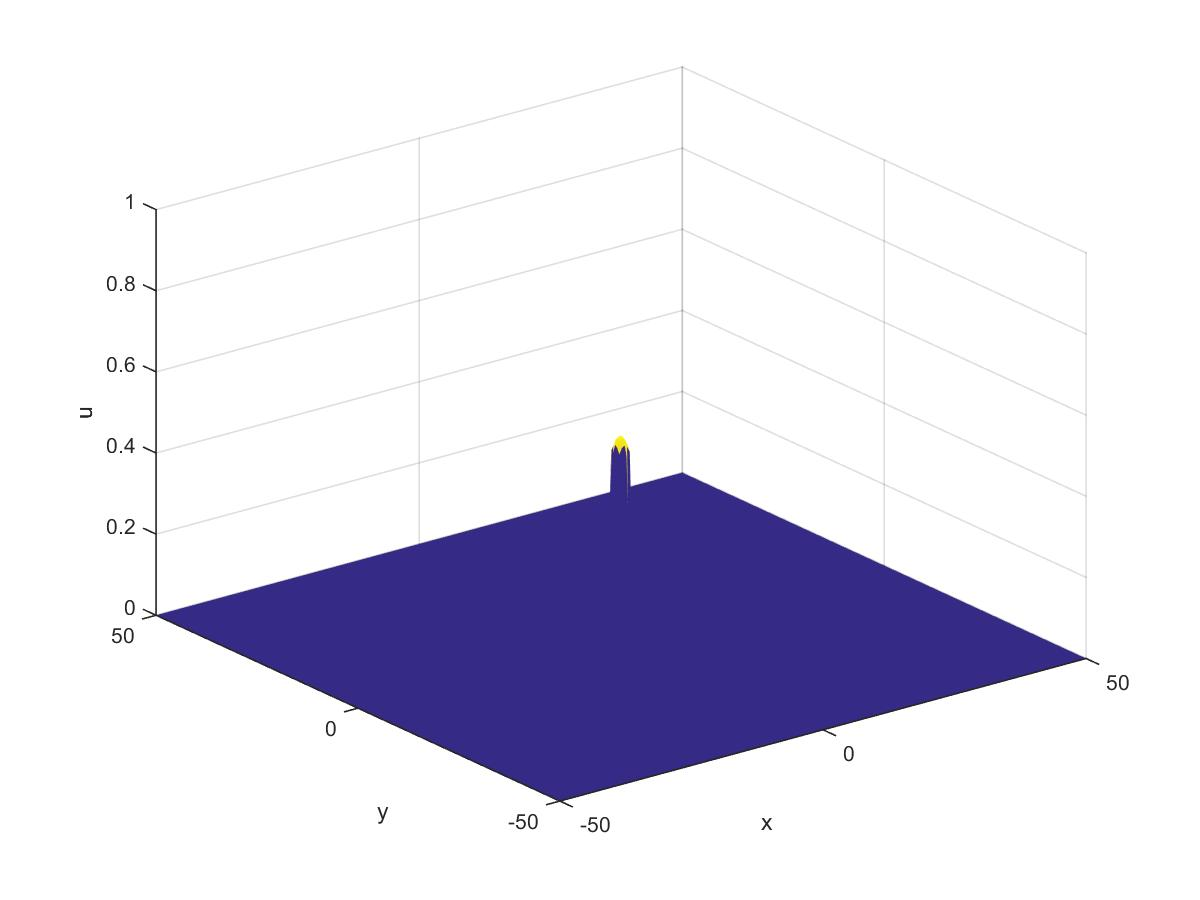
\includegraphics[width=0.3\linewidth]{Allee/322__1_}\hfill
    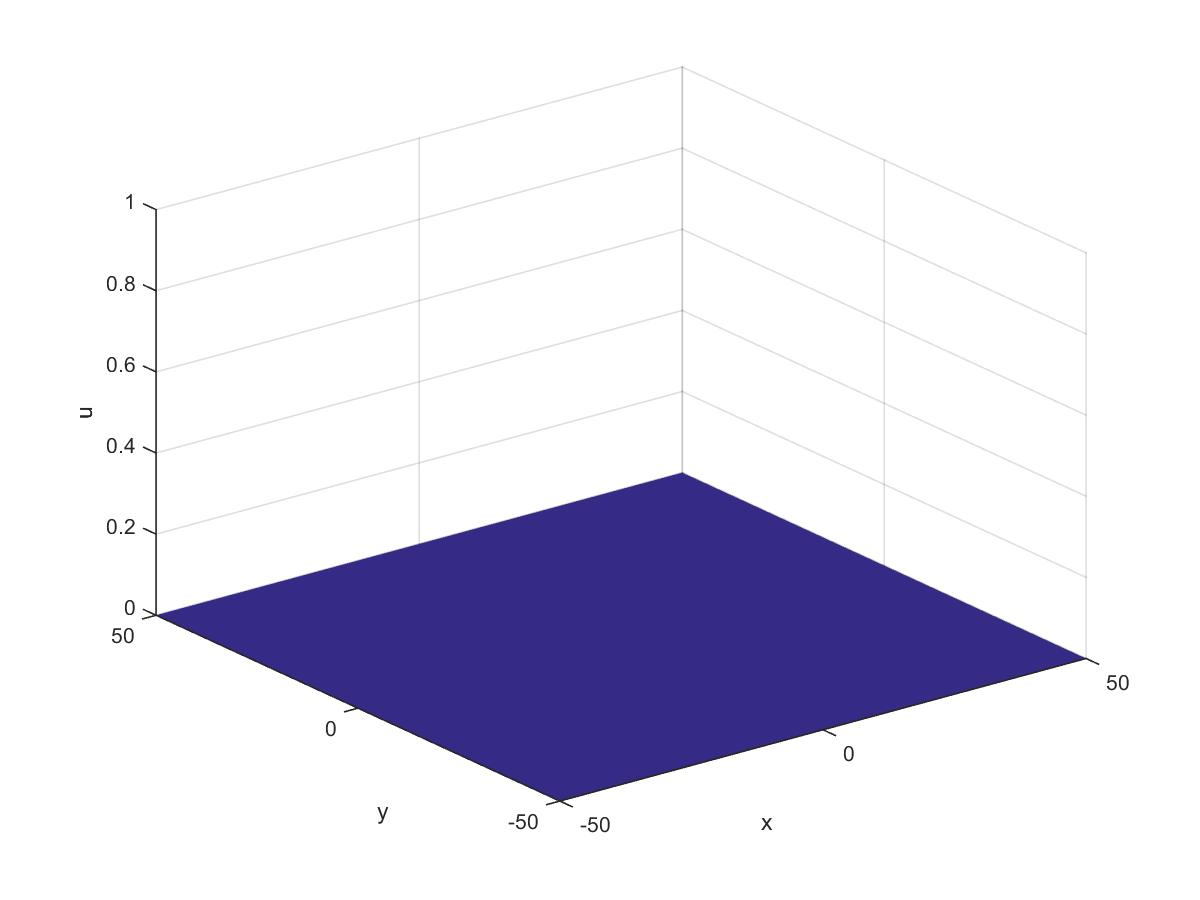
\includegraphics[width=0.3\linewidth]{Allee/322__2_}\hfill
	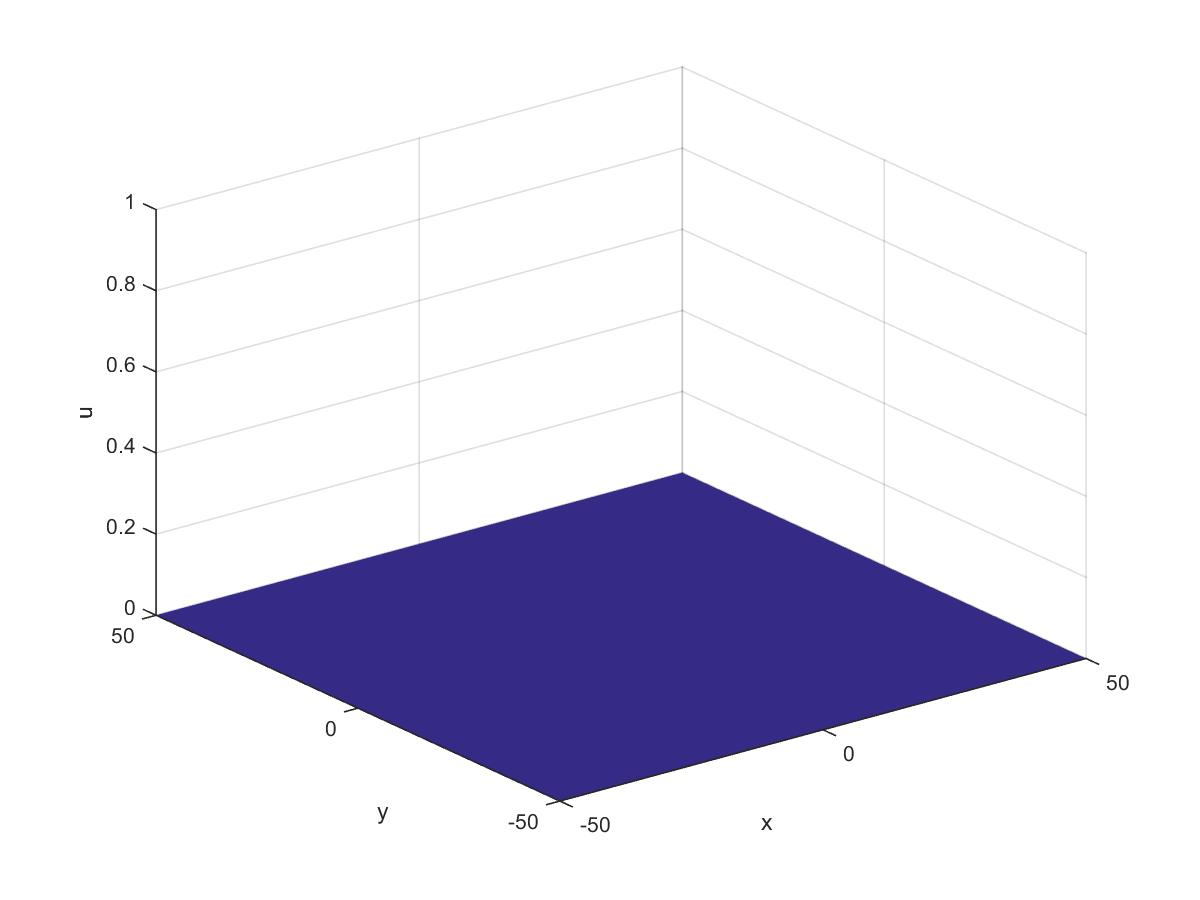
\includegraphics[width=0.3\linewidth]{Allee/322__3_}
\end{figure}
\end{frame}

\begin{frame}{$\ d=0.5, A=0.75 (k=7.1), u_0=0.9$}{}
\begin{figure}[H]
	\centering
	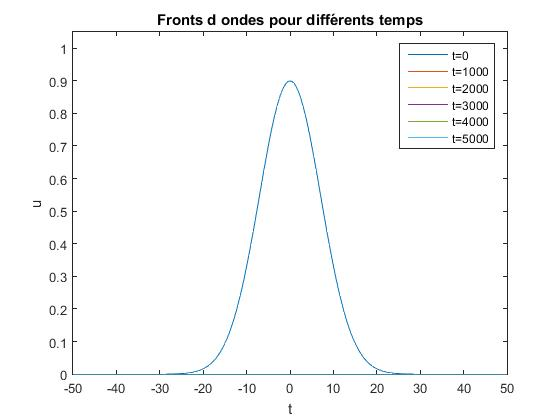
\includegraphics[width=0.40\linewidth, height=3cm]{Allee/F2323}\hfill
	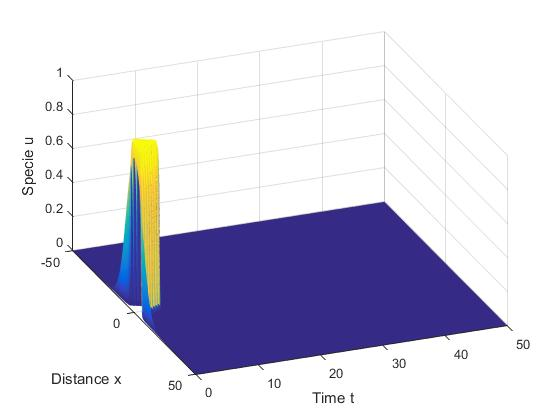
\includegraphics[width=0.55\linewidth, height=3cm]{Allee/F4323}
\end{figure}
\begin{figure}[H]
	\centering
	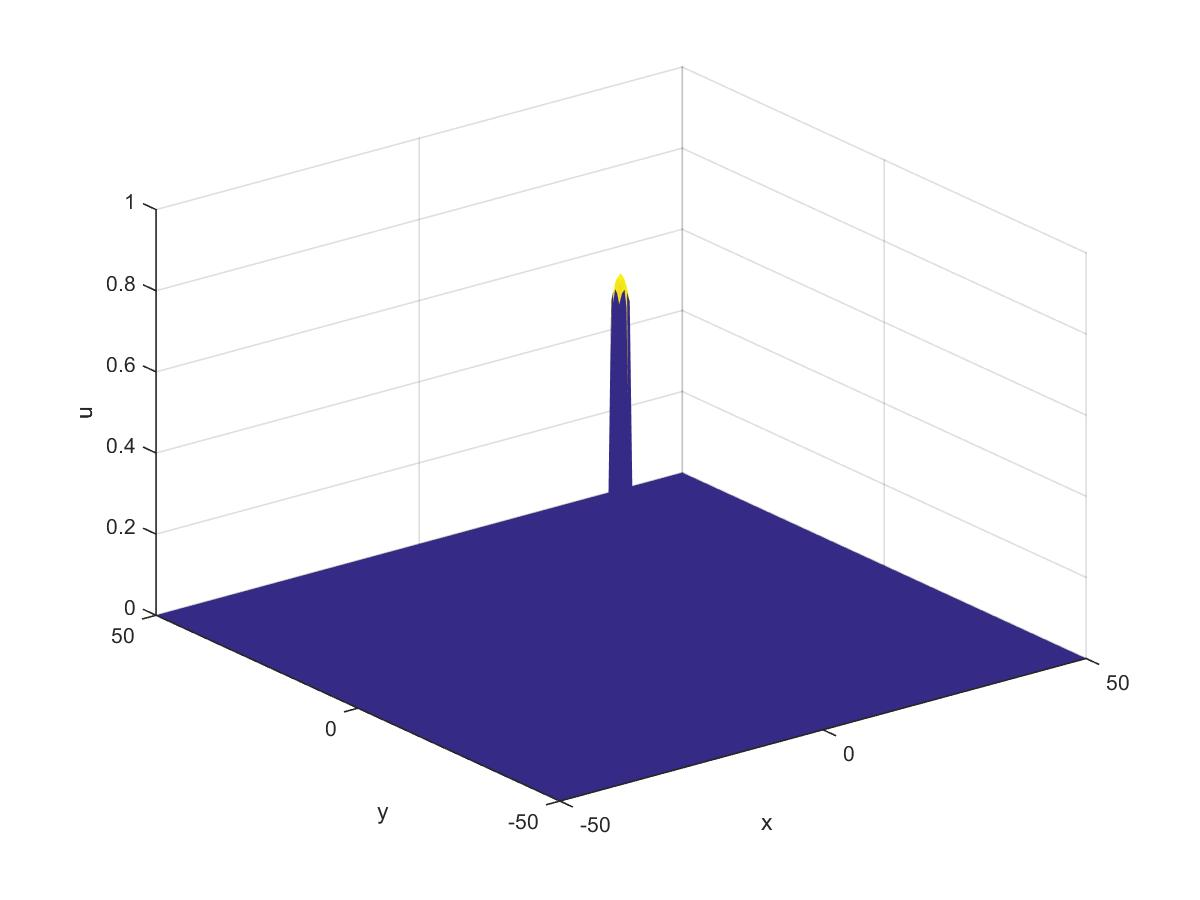
\includegraphics[width=0.3\linewidth]{Allee/323__1_}\hfill
    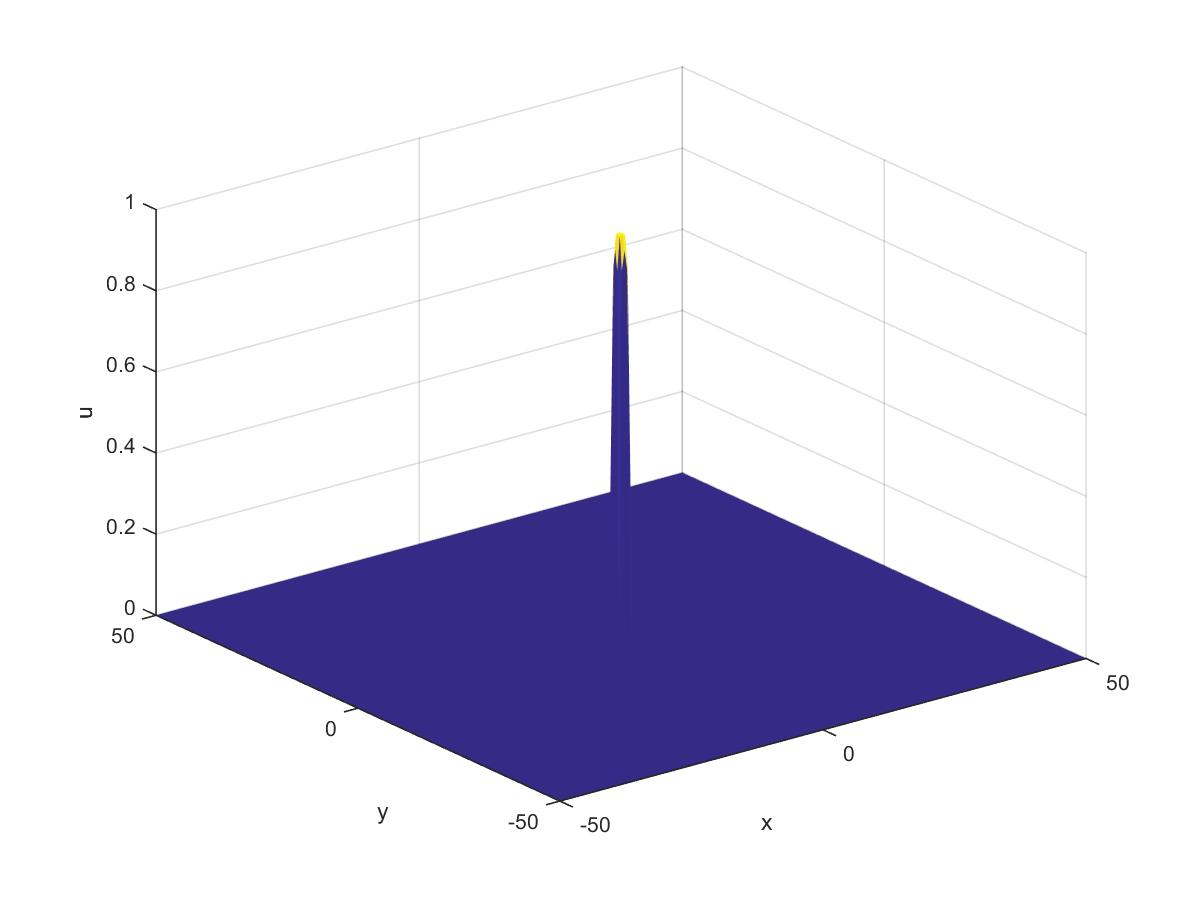
\includegraphics[width=0.3\linewidth]{Allee/323__2_}\hfill
	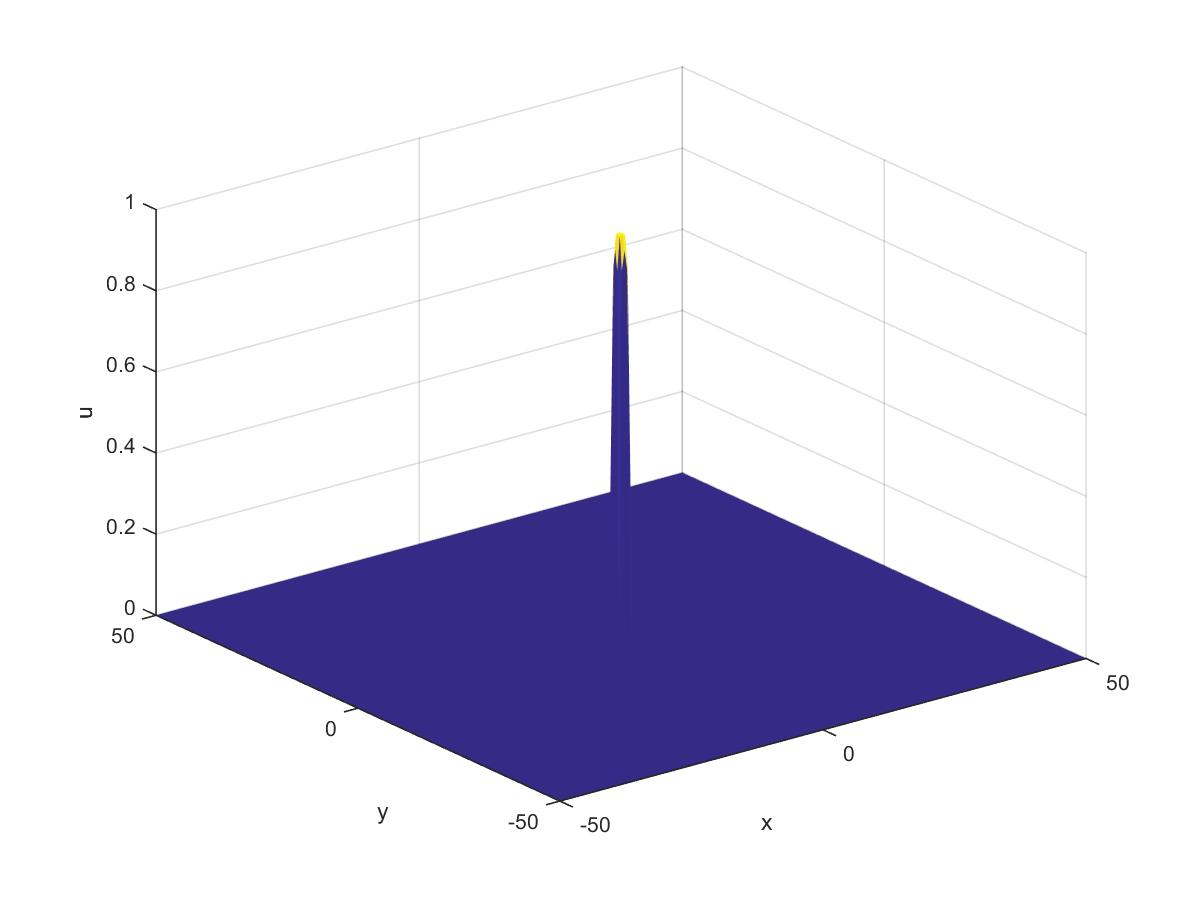
\includegraphics[width=0.3\linewidth]{Allee/323__3_}
\end{figure}
\end{frame}

\begin{frame}{$\ d=0.5, A=0.5 (k=16), u_0=0.1$}{}
\begin{figure}[H]
	\centering
	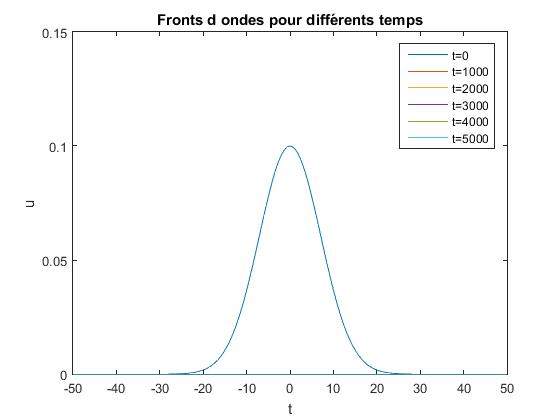
\includegraphics[width=0.40\linewidth, height=3cm]{Allee/F2331}\hfill
	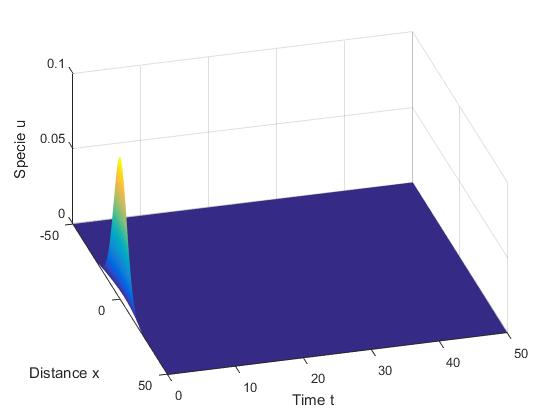
\includegraphics[width=0.55\linewidth, height=3cm]{Allee/F4331}
\end{figure}
\begin{figure}[H]
	\centering
	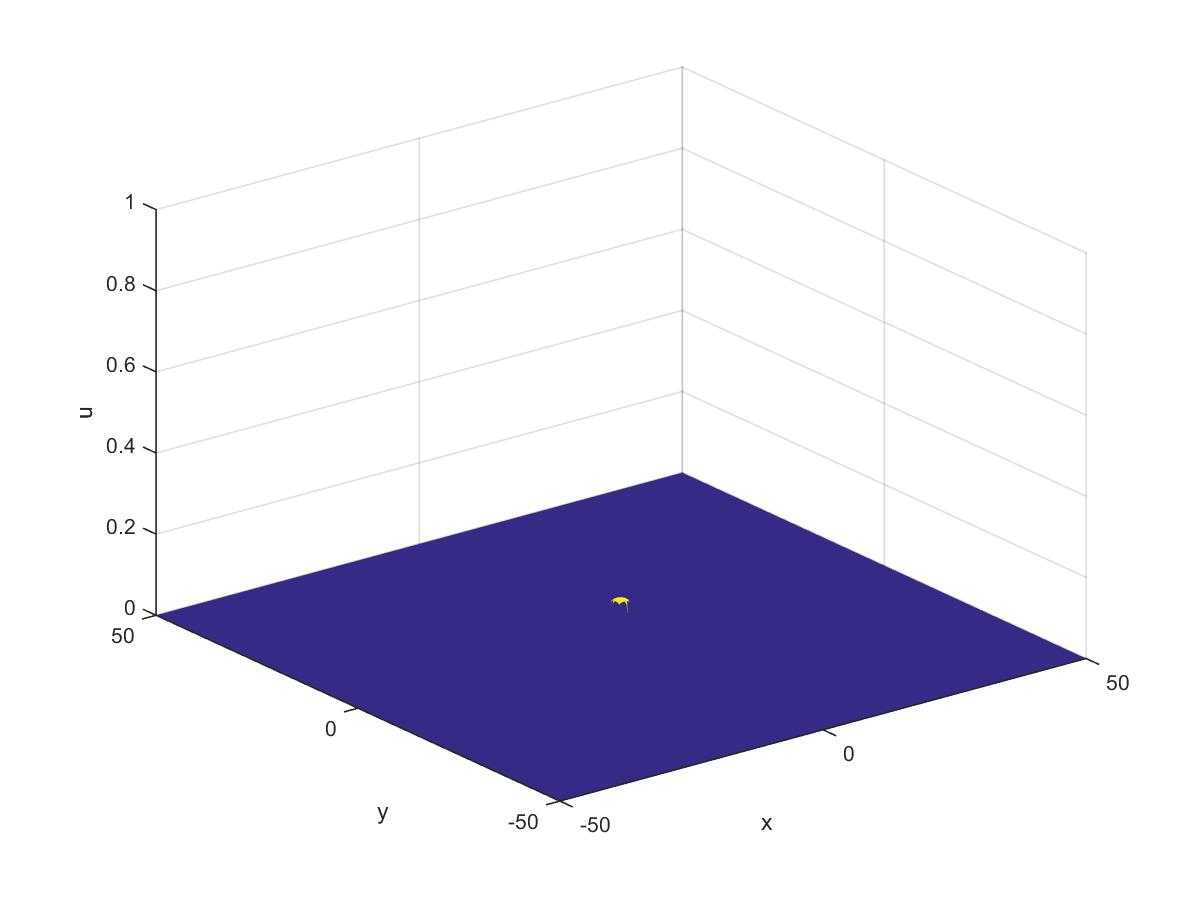
\includegraphics[width=0.3\linewidth]{Allee/331__1_}\hfill
    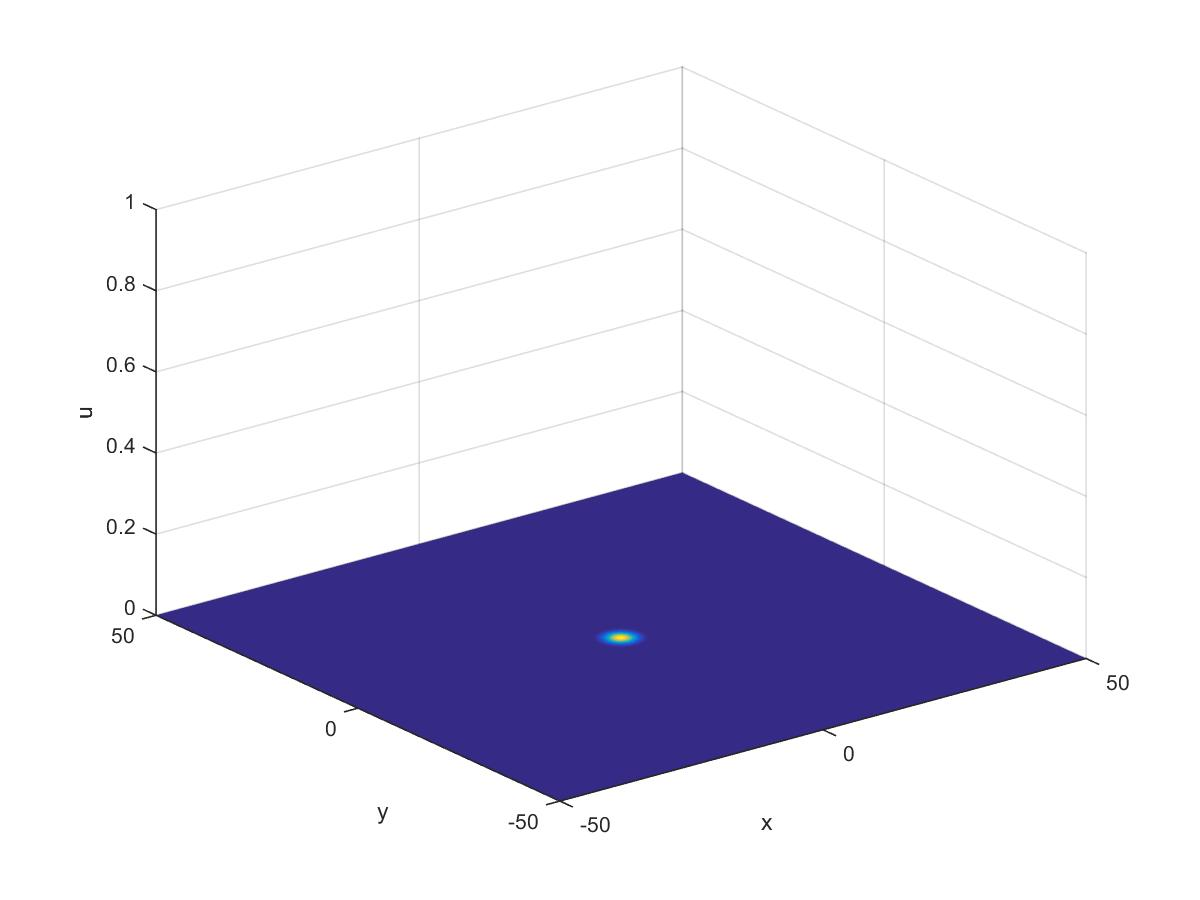
\includegraphics[width=0.3\linewidth]{Allee/331__2_}\hfill
	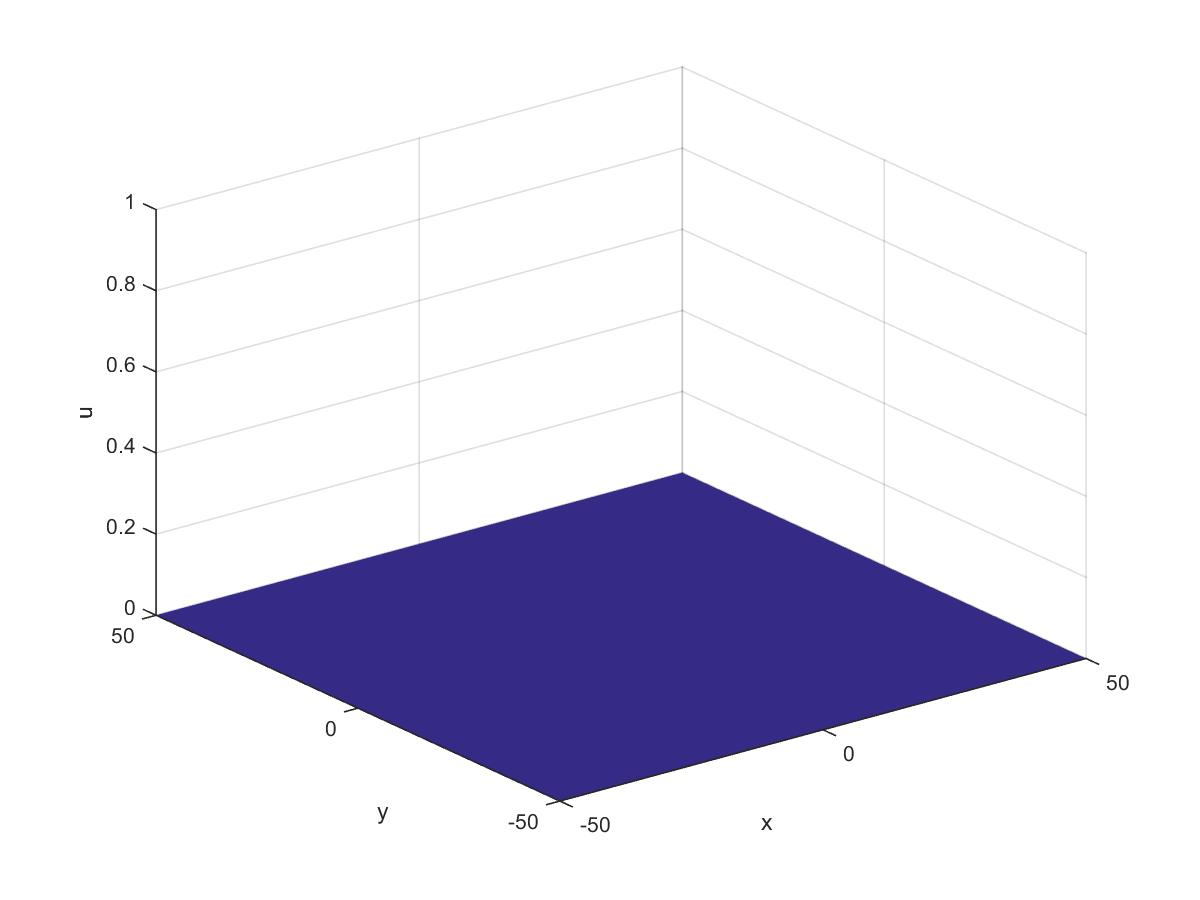
\includegraphics[width=0.3\linewidth]{Allee/331__3_}
\end{figure}
\end{frame}

\begin{frame}{$\ d=0.5, A=0.5 (k=16), u_0=0.9$}{}
\begin{figure}[H]
	\centering
	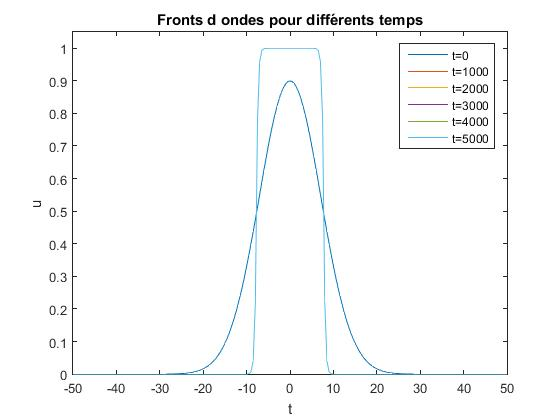
\includegraphics[width=0.40\linewidth, height=3cm]{Allee/F2333}\hfill
	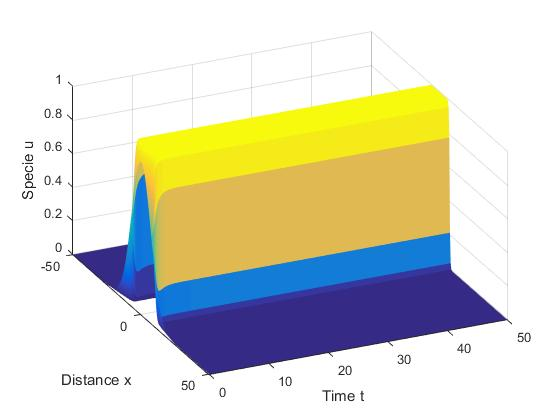
\includegraphics[width=0.55\linewidth, height=3cm]{Allee/F4333}
\end{figure}
\begin{figure}[H]
	\centering
	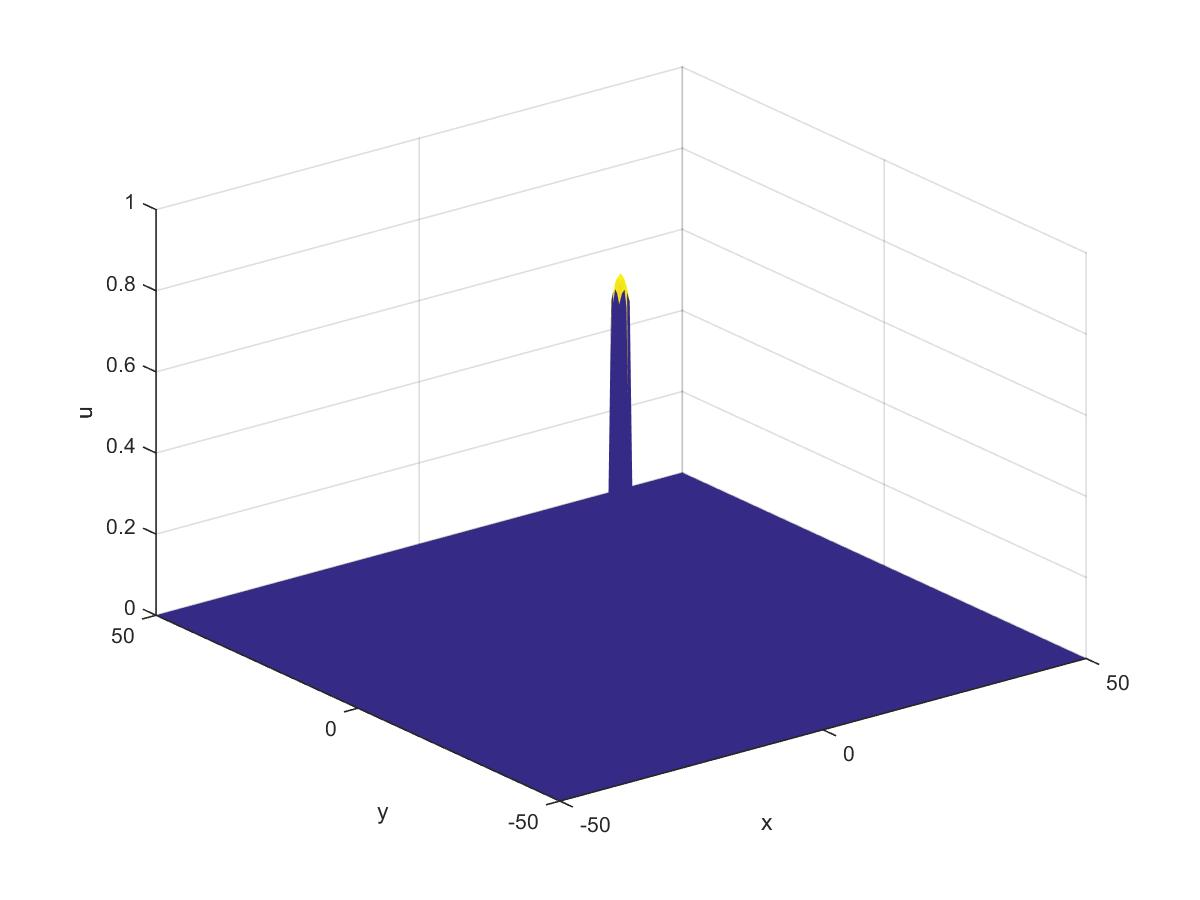
\includegraphics[width=0.3\linewidth]{Allee/333__1_}\hfill
    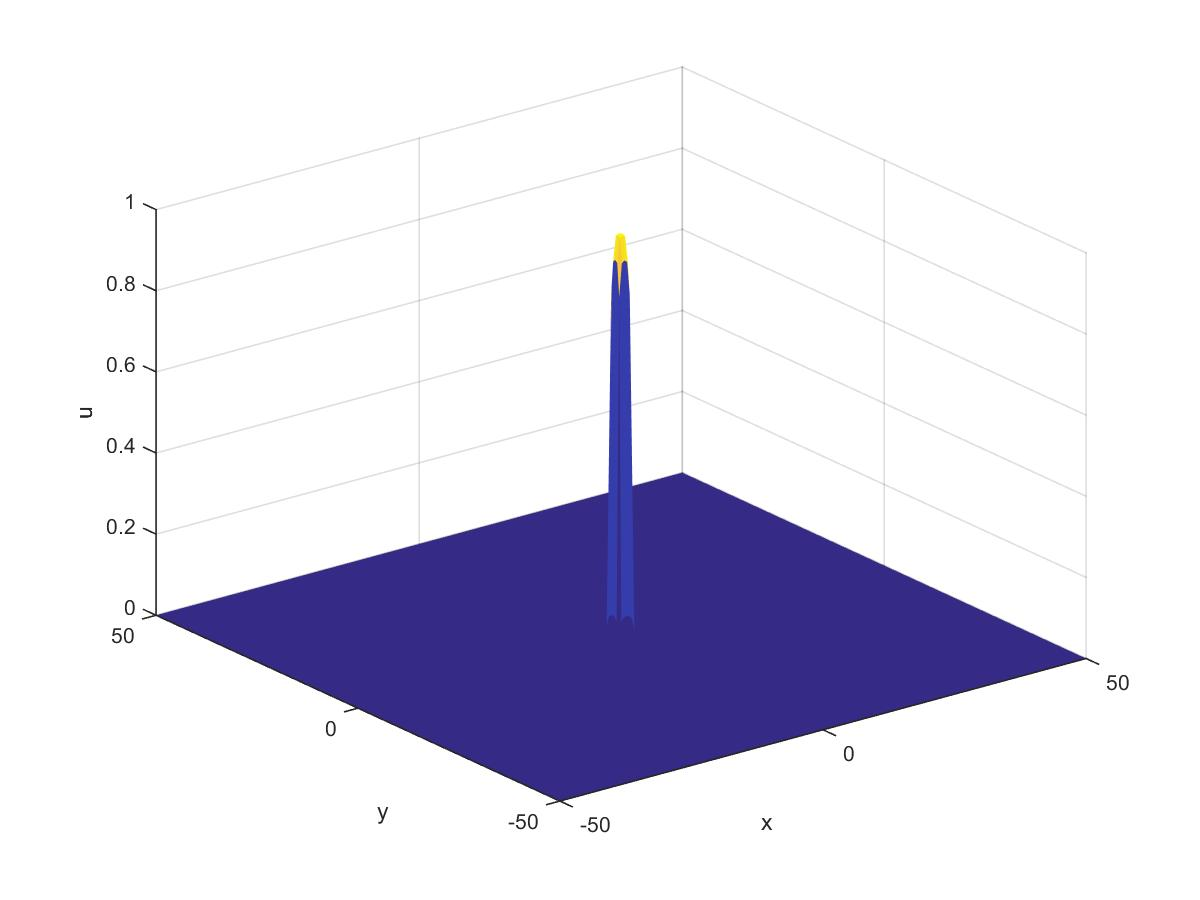
\includegraphics[width=0.3\linewidth]{Allee/333__2_}\hfill
	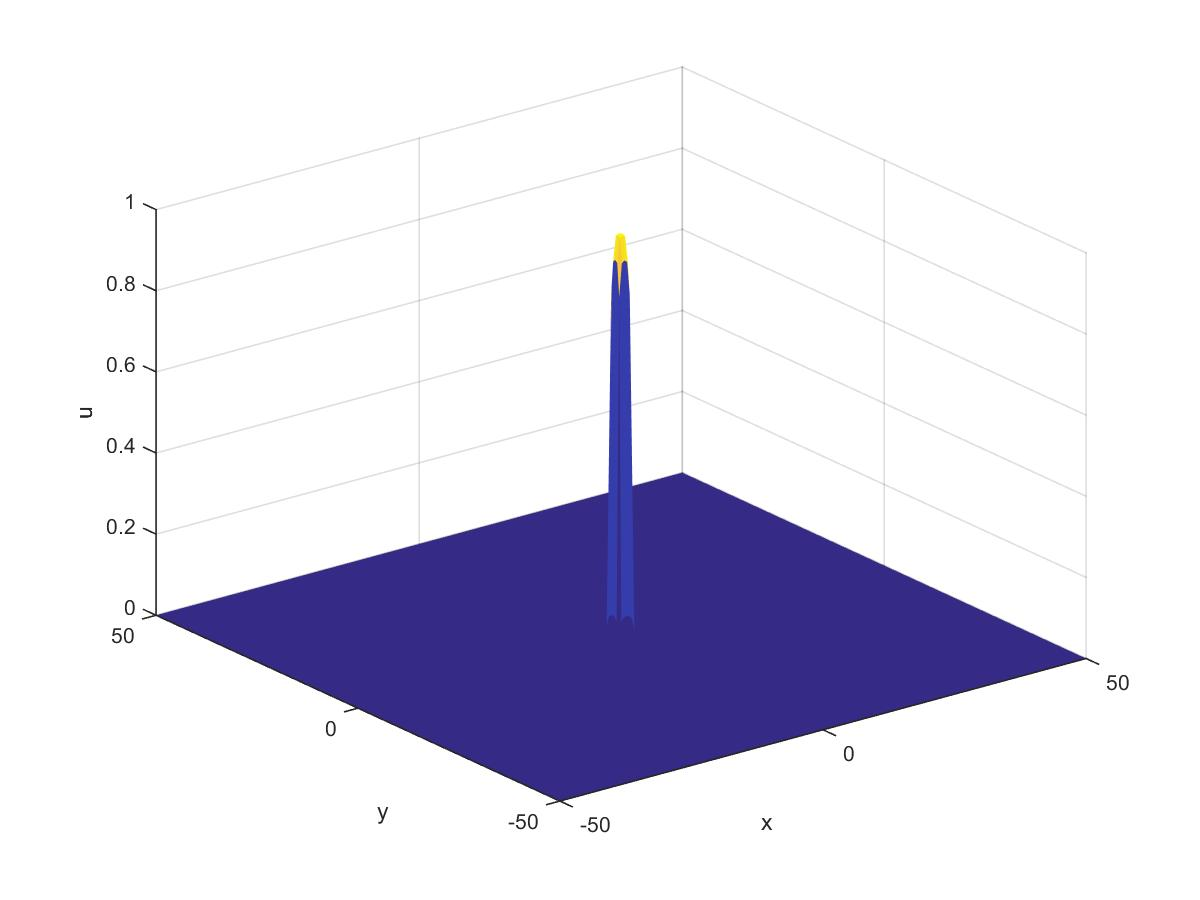
\includegraphics[width=0.3\linewidth]{Allee/333__3_}
\end{figure}
\end{frame}

\section{Système de Lotka-Volterra}
\subsection{Présentation du modèle}
\begin{frame}{Présentation du modèle}{}
\begin{block}{Modèle de compétition}
	$$\begin{cases} \frac{\partial u(t,x)}{\partial t} = f(u,v) + d_1\Delta u\\ \frac{\partial v(t,x)}{\partial t} = g(u,v) + d_2 \Delta v \\ 
\end{cases}$$
	$$f(u,v) = \alpha_1 u\left(1-\frac{u}{K_1}-\gamma_1\frac{v}{K_1}\right) \text{, } g(u,v) = \alpha_2 v\left(1-\frac{v}{K_2}-\gamma_2\frac{u}{K_2}\right)$$
\end{block}
\begin{itemize}
	\item u(t,x) : Densité de population des Hommes Modernes 
    \item v(t,x) : Densité de population des Hommes de Néanderthal 
    \item $K_1$ et $K_2$ : Capacités d'accueil du milieu
    \item $\gamma_1$ et $\gamma_2$ : Coefficients de compétition
    \item $\alpha_1$ et $\alpha_2$ : Taux de croissance
\end{itemize}
\end{frame}

\subsection{Analyse mathématique}
\begin{frame}{Analyse mathématique}{}
\begin{itemize}
\item[$\bullet$] On prend $\gamma_1 < \frac{K_1}{K_2}$ et $\gamma_2 > \frac{K_2}{K_1}$
\item[$\bullet$] Trois équilibres $(0,0)$, $(0,K_2)$, $(K_1,0)$.
\item[$\bullet$] En posant $\alpha = \alpha_1 = \alpha_2$, $K = K_1 = K_2$, $D = d_1 = d_2$ et $\gamma_1 + \gamma_2 = 2$ : existence de fronts d'ondes reliant 0 et K.
\item[$\bullet$] $c_{min} = 2 \sqrt{\alpha D(1-\gamma_1)}$
\end{itemize}
\end{frame}

\subsection{Simulations numériques}
\begin{frame}{Front d'ondes}{}
\begin{figure}[H]
\centering
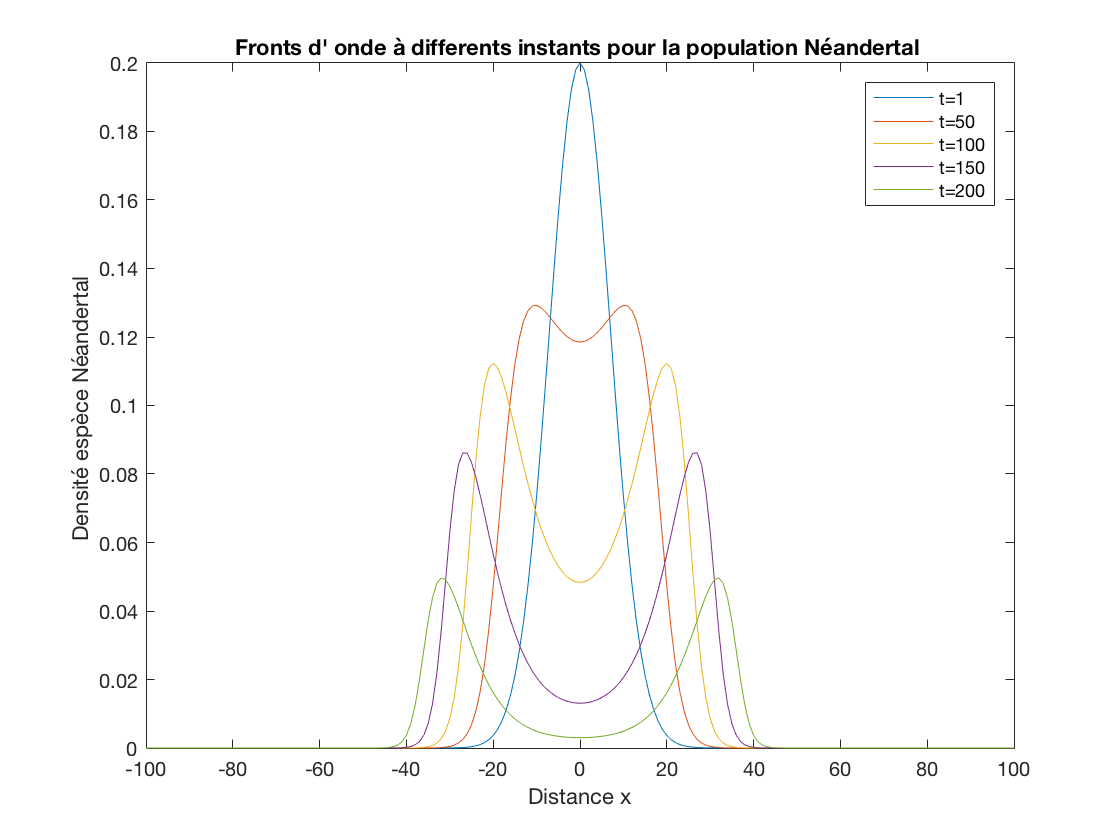
\includegraphics[width=0.48\linewidth]{Comp/neand.png}
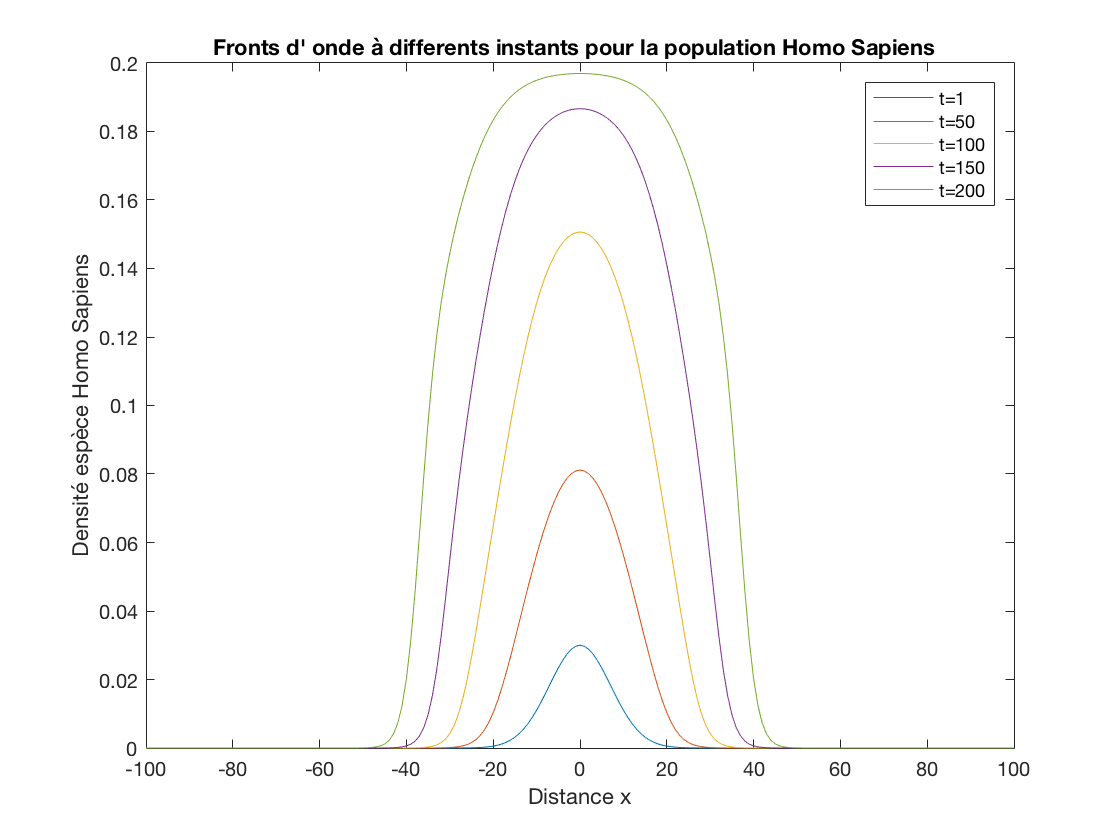
\includegraphics[width=0.48\linewidth]{Comp/homo.png}
\caption{Evolution des fronts d'onde au cours du temps (\url{Competition.avi} )}
\end{figure}
\end{frame}

\begin{frame}{Diffusion 1D}{}
\begin{figure}[H]
\centering
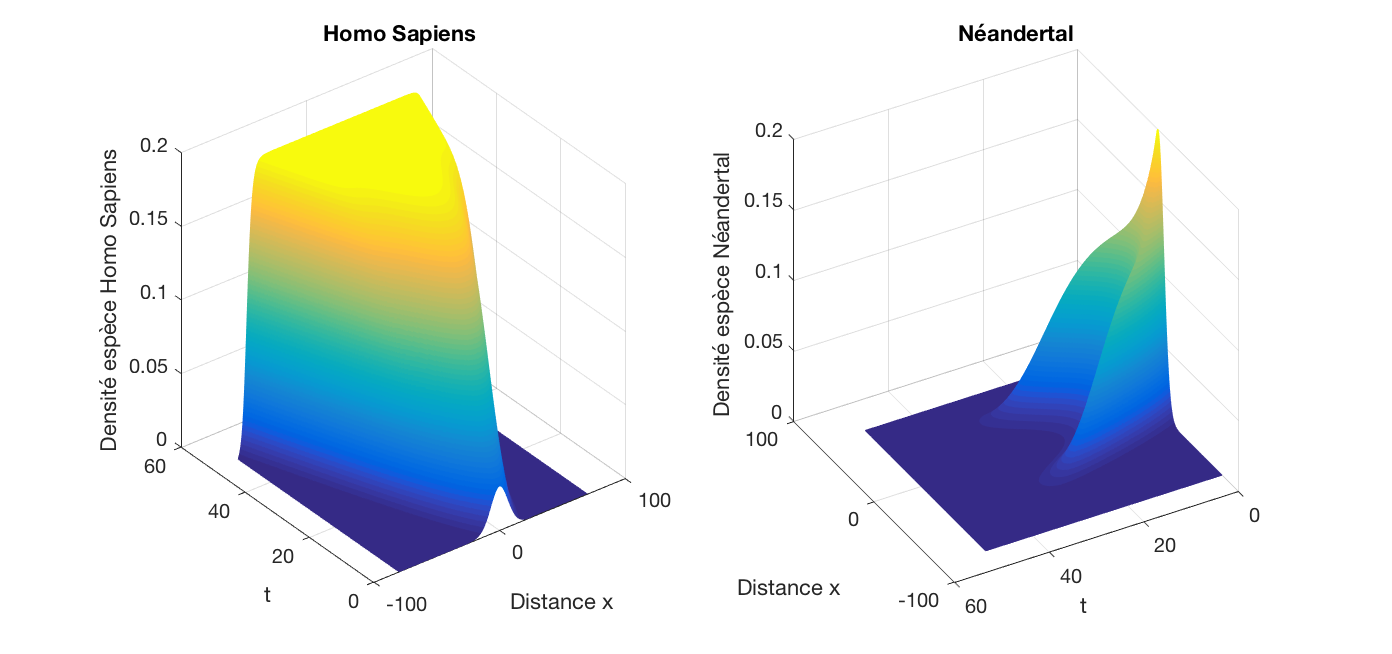
\includegraphics[scale=0.2]{Comp/CompDiff2.png}
\caption{Diffusion 1D}
\end{figure}
\end{frame}

\section{Conclusion}


\end{document}